\documentclass[12pt,a4paper,twoside,openright]{llncs}

               %%%%%%%%%%%%%%%%%%%%%%%%%%%%%%%%%%%%%%
               %    Scelta dei package da usare     %
               %%%%%%%%%%%%%%%%%%%%%%%%%%%%%%%%%%%%%%

\usepackage[utf8]{inputenc}
%%\usepackage{amsmath,amsfonts,amssymb,amsthm}
\usepackage[english]{babel}
\usepackage[T1]{fontenc}
\usepackage{url}
\usepackage{xspace}
\usepackage{fancyhdr}
\usepackage{graphicx}
\usepackage{eurosym}
\usepackage{afterpage}
\usepackage{float}
\usepackage{wrapfig}
\usepackage{lscape}
\usepackage{rotating}
\usepackage{epstopdf}

\input{jsonListing.tex}


\makeatletter

\usepackage{manifest}

\makeatother

               %%%%%%%%%%%%%%%%%%%%%%%%%%%%%%%%%%%%%%%%
               % Scelta delle dimensioni della pagina %
               %%%%%%%%%%%%%%%%%%%%%%%%%%%%%%%%%%%%%%%%

\setlength{\textwidth}{13.5cm}
\setlength{\textheight}{19cm}
\setlength{\footskip}{3cm}
\setlength{\parskip}{0.5em}
\setlength{\parindent}{1em}

               %%%%%%%%%%%%%%%%%%%%%%%%%%%%%%%%%%%%
               %    Reduce Section Spaceing       %
               %%%%%%%%%%%%%%%%%%%%%%%%%%%%%%%%%%%%

%% sudo apt-get install texlive-latex-extra required.


%% Save the class definition of \subparagraph
\let\llncssubparagraph\subparagraph
%% Provide a definition to \subparagraph to keep titlesec happy
\let\subparagraph\paragraph
%% Load titlesec
\usepackage[compact]{titlesec}
%% Revert \subparagraph to the llncs definition
\let\subparagraph\llncssubparagraph

\titlespacing{\section}{0pt}{2ex}{1ex}
\titlespacing{\subsection}{0pt}{1ex}{0ex}
\titlespacing{\subsubsection}{0pt}{0.5ex}{0ex}

               %%%%%%%%%%%%%%%%%%%%%%%%%%%%%%%%%%%%%
               % Commands inseriti per il template %
               %               di Natali           %
               %%%%%%%%%%%%%%%%%%%%%%%%%%%%%%%%%%%%%

\newcommand{\java}{\textsf{Java}}
\newcommand{\contact}{\emph{Contact}}
\newcommand{\corecl}{\texttt{corecl}}
\newcommand{\medcl}{\texttt{medcl}}
\newcommand{\msgcl}{\texttt{msgcl}}
\newcommand{\android}{\texttt{Android}}
\newcommand{\dsl}{\texttt{DSL}}
\newcommand{\jazz}{\texttt{Jazz}}
\newcommand{\rtc}{\texttt{RTC}}
\newcommand{\ide}{\texttt{Contact-ide}}
\newcommand{\xtext}{\texttt{XText}}
\newcommand{\xpand}{\texttt{Xpand}}
\newcommand{\xtend}{\texttt{Xtend}}
\newcommand{\pojo}{\texttt{POJO}}
\newcommand{\junit}{\texttt{JUnit}}

\newcommand{\action}[1]{\texttt{#1}\xspace}
\newcommand{\code}[1]{{\small{\texttt{#1}}}\xspace}
\newcommand{\codescript}[1]{{\scriptsize{\texttt{#1}}}\xspace}

% Cross-referencing
\newcommand{\labelsec}[1]{\label{sec:#1}}
\newcommand{\xs}[1]{\sectionname~\ref{sec:#1}}
\newcommand{\xsp}[1]{\sectionname~\ref{sec:#1} \onpagename~\pageref{sec:#1}}
\newcommand{\labelssec}[1]{\label{ssec:#1}}
\newcommand{\xss}[1]{\subsectionname~\ref{ssec:#1}}
\newcommand{\xssp}[1]{\subsectionname~\ref{ssec:#1} \onpagename~\pageref{ssec:#1}}
\newcommand{\labelsssec}[1]{\label{sssec:#1}}
\newcommand{\xsss}[1]{\subsectionname~\ref{sssec:#1}}
\newcommand{\xsssp}[1]{\subsectionname~\ref{sssec:#1} \onpagename~\pageref{sssec:#1}}
\newcommand{\labelfig}[1]{\label{fig:#1}}
\newcommand{\xf}[1]{\figurename~\ref{fig:#1}}
\newcommand{\xfp}[1]{\figurename~\ref{fig:#1} \onpagename~\pageref{fig:#1}}
\newcommand{\labeltab}[1]{\label{tab:#1}}
\newcommand{\xt}[1]{\tablename~\ref{tab:#1}}
\newcommand{\xtp}[1]{\tablename~\ref{tab:#1} \onpagename~\pageref{tab:#1}}
% Category Names
\newcommand{\sectionname}{Section}
\newcommand{\subsectionname}{Subsection}
\newcommand{\sectionsname}{Sections}
\newcommand{\subsectionsname}{Subsections}
\newcommand{\secname}{\sectionname}
\newcommand{\ssecname}{\subsectionname}
\newcommand{\secsname}{\sectionsname}
\newcommand{\ssecsname}{\subsectionsname}
\newcommand{\onpagename}{on page}

               %%%%%%%%%%%%%%%%%%%%%%%%%%%%%%%%%%%%%%%%
               % Informazioni generali sul dacumento  %
               %    da usare nell'intestazione        %
               %%%%%%%%%%%%%%%%%%%%%%%%%%%%%%%%%%%%%%%%

\newcommand{\xauthA}{Name1 Surename1}
\newcommand{\xauthB}{Name2 Surename2}
\newcommand{\xauthC}{Name3 Surename3}
\newcommand{\xfaculty}{II Faculty of Engineering}
\newcommand{\xunibo}{Alma Mater Studiorum -- University of Bologna}
\newcommand{\xaddrBO}{viale Risorgimento 2}
\newcommand{\xaddrCE}{via Venezia 52}
\newcommand{\xcityBO}{40136 Bologna, Italy}
\newcommand{\xcityCE}{47023 Cesena, Italy}

\setcounter{tocdepth}{3}
\setcounter{secnumdepth}{3}

\begin{document}

%%%%%%%%%%%%%%%%%%%%%%%%%%%%%%%%%%%%%%%%
%  Inserimento della pagina iniziale   %
%%%%%%%%%%%%%%%%%%%%%%%%%%%%%%%%%%%%%%%%

\title{Project Report Template}

%%% \author{\xauthA \and \xauthB}
\author{\xauthA \and \xauthB \and \xauthC}

%
%%%  \xunibo\\\xaddrCE, \xcityCE\\\email{\{nameA.studentA, nameB.studentB\}@studio.unibo.it}
\institute {  \xunibo\\\xaddrCE, \xcityCE\\\email{\{name1.surename1, name2.surename2, name3.surename3\}@mail.com }}

\maketitle

\tableofcontents

\newpage
%%%%%%%%%%%%%%%%%%%%%%%%%%%%%%%%%%%%%%%%%%%
% inclusione dei capitoli e intestazione  %
%%%%%%%%%%%%%%%%%%%%%%%%%%%%%%%%%%%%%%%%%%%

\section{Introduzione}
\labelsec{intro}

Questo \'e il template di progetto del corso di smart city dell'universit\'a di Bologna. Di seguito sar\'a consultabile tutto il processo di analisi del progetto: modelli, problemi riscontrati e soluzioni adottate, interazione con l'ambiente, sensori utilizzati e il loro collegamento \ldots

Per qualsiasi dubbio in merito fare riferimento agli autori.


\section{Visione}
\labelsec{Visione}

La visione che guida questo progetto consiste nel raggiungere rapidamente l'ideale di città intelligente, quindi con un ambiente aumentato, capace di prendere decisioni e agire tempestivamente per far fronte a casi specifici e capace di comunicare direttamente con chi si trova immerso in esso, per facilitare la vita di tutti i giorni. 

In particolare vogliamo prepararci ad imparare, modellare e costruire sistemi che si integreranno in questo contesto, visto l'andamento stesso del mercato che sta sempre più rendendo disponibili risorse di elaborazione e sensoristica a minor prezzo.


\section{Obbiettivi}
\labelsec{Goals}

Lo scopo del progetto \'e quello di implementare concretamente un'applicazione di domotica. Affrontando quindi tutte le problematiche ad essa annesse e fornire una possibile soluzione a queste. Ci auguriamo che questa possa essere di spunto per applicazioni simili e che possa quindi favorirne lo sviluppo.

Sfruttando questo progetto, vogliamo esplorare e apprendere la teoria e i concetti affrontati nel corso di smart city. Quindi tutti gli aspetti riguardanti la gestione di sensori e input provenienti dall'ambiente esterno. Uscendo dalla tipica zona di confort dei sistemi software.


\newpage




\section{Requisiti}
\labelsec{Requirements}

Si vuole monitorare lo stato ambientale di una stanza. In particolare si vogliono monitorare lo stato di: luce, temperatura, umidit\`a, gas e movimento, mantenendo la possibilit\`a di aggiungere altre tipologie di sensori.

Il sistema dovr\`a dare all'utente la possibilit\`a di inserire, attraverso un'interfaccia web, per ogni tipologia di dato, un'apposito range che indichi i valori ammessi all'interno della stanza in modo che, in caso uno dei valori misurati non risulti conforme alle specifiche, venga indicata una notifica di allarme sull'interfaccia stessa. Questo con l'idea di simulare la possibilit\`a di eseguire delle azioni collegate all'allarme (ad esempio, accensione delle luci o del riscaldamento)

L'utente potr\`a inoltre visualizzare all'interno del sito i valori misurati in tempo reale e il valore dei vari sensori nel tempo.

\subsection{Requisiti Non Funzionali}

Aggiungiamo nei requsiti non funzionali tutte le propriet\`a che il sistema deve avere e che non sono state ufficialmente formalizzate.

\begin{itemize}
  \item Separazione dei compiti e indipendenza tra le parti: garantire i principi SOLID dove \`e possibile evitare che un qualsiasi componente sia strettamente legato ad un'altro.
  \item Reattivit\`a: si visualizzi il Reactive Manifesto per i dettagli delle propriet\`a.
\end{itemize}


\section{Acquisto Hardware}
\labelsec{Hardware Procurement}

Sfortunatamente il primo problema incontrato in un progetto come il seguente \`e stata la necessit\`a di acquistare la parte hardware del sistema che si andr\` a costruire. Di consequenza si \`e messo in atto un processo di ricerca dei sensori, cavi e quant'altro per riuscire a soddisfare i requisiti

\subsection{Dispositivi di Computazione}

Prima di tutto necessitiamo di un dispositivo in grado di computare i dati emessi dai vari sensori e che sia interamente programmabile. Nel corso abbiamo visto due possibilit\`a che hanno avuto molto successo recentemente:

\begin{itemize}
  \item Arduino
  \item Raspberry Pi
\end{itemize}

Abbiamo scelto la seconda opzione data la maggior familiarit\`a con il dispositivo e dal momento in cui risulta piu' facile il riutilizzo dello stesso una volta terminato questo progetto.

\begin{figure}
	\centering
	\includegraphics[width=0.7\linewidth]{Figures/Sensors&Rasp/Pi2}
	\caption[raspberry]{Scheda del Raspberry 2}
	\label{fig:Pi2}
\end{figure}

IIl Rasberry Pi 2 (figura~\ref{fig:Pi2}) è un SoC (sistema integrato) cio\`e possiede un chip che integra al suo interno processore, chipset, RAM ed eventuale circuteria input/output. \`E dotato delle seguenti uscite:

\begin{itemize}
	\item USB 2.0 (4)
	\item Ethernet
	\item HDMI
	\item Aux
	\item DC (Alimentazione)
	\item Slot MicroSD
\end{itemize}
Infine dispone di un GPIO (General Purpose Input/Output) interfaccia attraverso la quale è possibile comunicare con sensori esterni per mezzo di segnali digitali ed interagire con l'ambiente esterno.

Costo del dispositivo: 44,50 \euro


\subsection{Sensori}

Un'altra cosa fondamentale riguarda i sensori necessari per catturare i parametri richiesti.
Tutti i sensori per standard possono lavorare con una tensione di 5v.
Ogni sensore possiede 3 o 4 pin:

\begin{itemize}
	\item Vcc: Pin di alimentazione
	\item GND: Pin della massa
	\item Dout: Porta input/output digitale
	\item Aout: Porta input/output analogica (opzionale)
\end{itemize}

 Abbiamo Quindi scelto i sequenti sensori:

\begin{table}[]
	
	\begin{tabular}{lllll}
		\cline{1-3}
		\multicolumn{1}{|l|}{Parametri Ambientali} & \multicolumn{1}{l|}{Sensori} & \multicolumn{1}{l|}{Costo} &  &  \\ \cline{1-3}
		Temperatura \& Umidità                     & DHT11                        & 6\euro                          &  &  \\
		Luminosità                                 & Light                        & 5\euro                          &  &  \\
		Movimento                                  & HC-SR501                     & 6\euro                          &  &  \\
		Gas                                  & MQ-2                   & 7\euro                         &  &
	\end{tabular}
	\centering
	\caption{Sensor table}
	\label{my-label}

\end{table}


\newpage

\begin{figure}
\centering
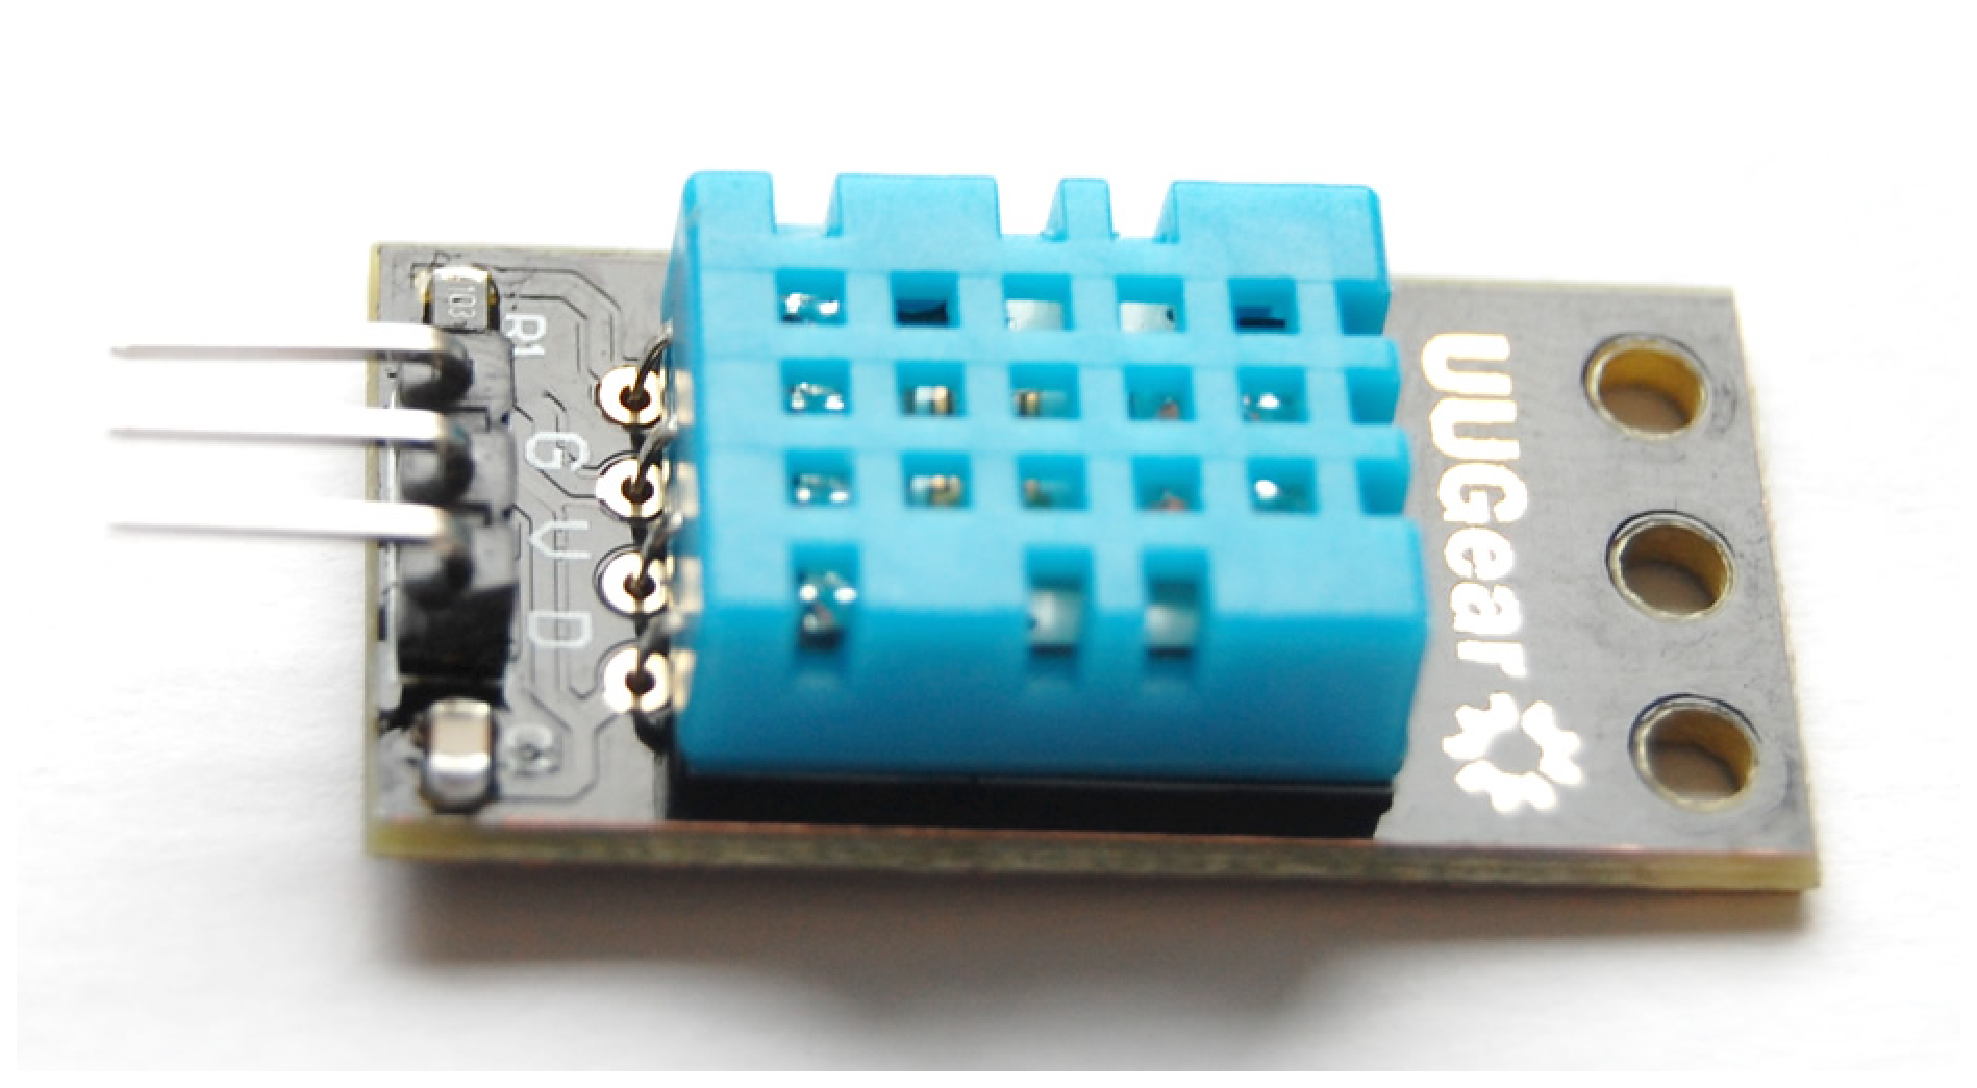
\includegraphics[width=0.7\linewidth]{Figures/Sensors&Rasp/dht11}
\caption[dht11]{DHT11 Sensor}
\label{fig:dht11}
\end{figure}

 Il sensore DHT11 (figura~\ref{fig:dht11}) \`e in grado rilevare la temperatura e l'umidità dell'ambiente circostante. Possiede tre Pin per interfacciarsi.
 Le sue caratteristiche tecniche sono:
 
 \begin{itemize}
 	\item Vcc: 3.3$\sim$5.5V
 	\item Range: Temperatura 0 \textasciitilde 50℃, Umidità:  20-90%RH
 	\item Accuratezza: Temperatura +-2℃, Umidit\`a +-5%RH
 	\item Risoluzione: Temperatura  1℃, Umidit\`a  1%RH
 \end{itemize}
 
 \newpage
 
\begin{figure}
	\centering
	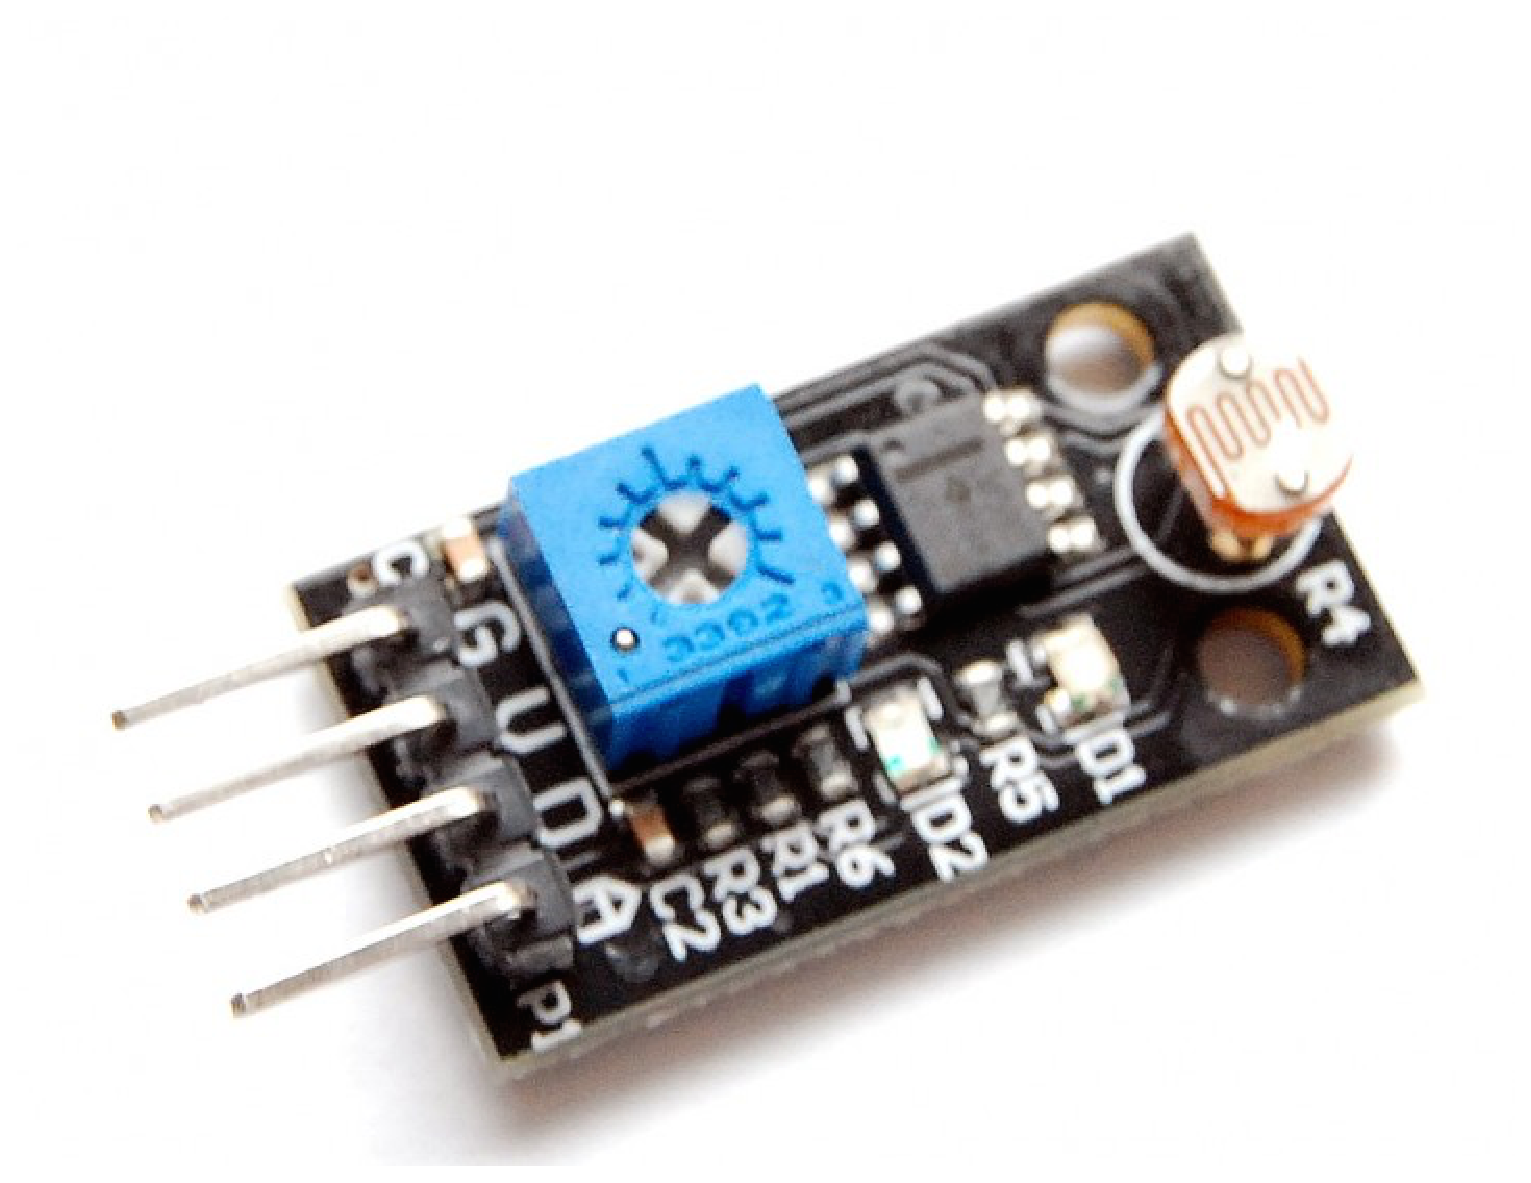
\includegraphics[width=0.7\linewidth]{Figures/Sensors&Rasp/light}
	\caption[light]{Light Sensor}
	\label{fig:light}
\end{figure}


Il sensore di luminosit\`a (figura~\ref{fig:light} ) \`e un sensore dotato di un fotoresistore (componente circolare posizionato in fondo al circuito), un trimmer e due led. Il trimmer (equivalente ad un potenziometro) permette di regolare la sensibilità alla luce del sensore. Un led rimane costantemente acceso per indicare che il sensore \`e correttamente alimentato ed in funzione, l'altro si accende o si spegne nel momento in cui la luce percepita dal fotoresistore risulta sotto o sopra la soglia. Il sensore possiede quattro Pin per interfacciarsi.
Le sue caratteristiche tecniche sono:

\begin{itemize}
	\item Vcc: 3.3$\sim$5.5V
	\item Output: HIGH o LOW (boolean sensor: 0-1)
\end{itemize}

\newpage

\begin{figure}
	\centering
	\includegraphics[width=0.7\linewidth]{Figures/Sensors&Rasp/pir}
	\caption[PIR] {HC-SR501 Sensor}
	\label{fig:pir}
\end{figure}

Il sensore di prossimit\`a (figura~\ref{fig:pir}) permette di individuare gli spostamenti in una determinata area. Il suo funzionamento \`e dato da un componente chiamato "PIR" (Passive InfraRed) che per mezzo dei raggi infrarossi emanati dagli oggetti in uno spazio \`e in grado di percepire variazioni di movimento. Vi sono inoltre due trimmer arancioni per permettere di regolare il range di movimento e il tempo di delay. La semisfera di plastica trasparente posta sopra al modulo serve per poter massimizzare l'area di visibilità del sensore. Questa infatti, al suo interno, possiede particolari scanalature per che permettono di ridirigere correttamente i raggi al sensore. Vi sono tre Pin per interfacciarsi.
Le sue caratteristiche tecniche sono:

\begin{itemize}
	\item Vcc: 5$\sim$20V
	\item Range: 5~7 metri
	\item Ampiezza: ~120°
	\item Tempo di delay : 0.3-600 secondi
	\item Output: HIGH o LOW (boolean sensor: 0-1)
\end{itemize}


\begin{figure}
	\centering
	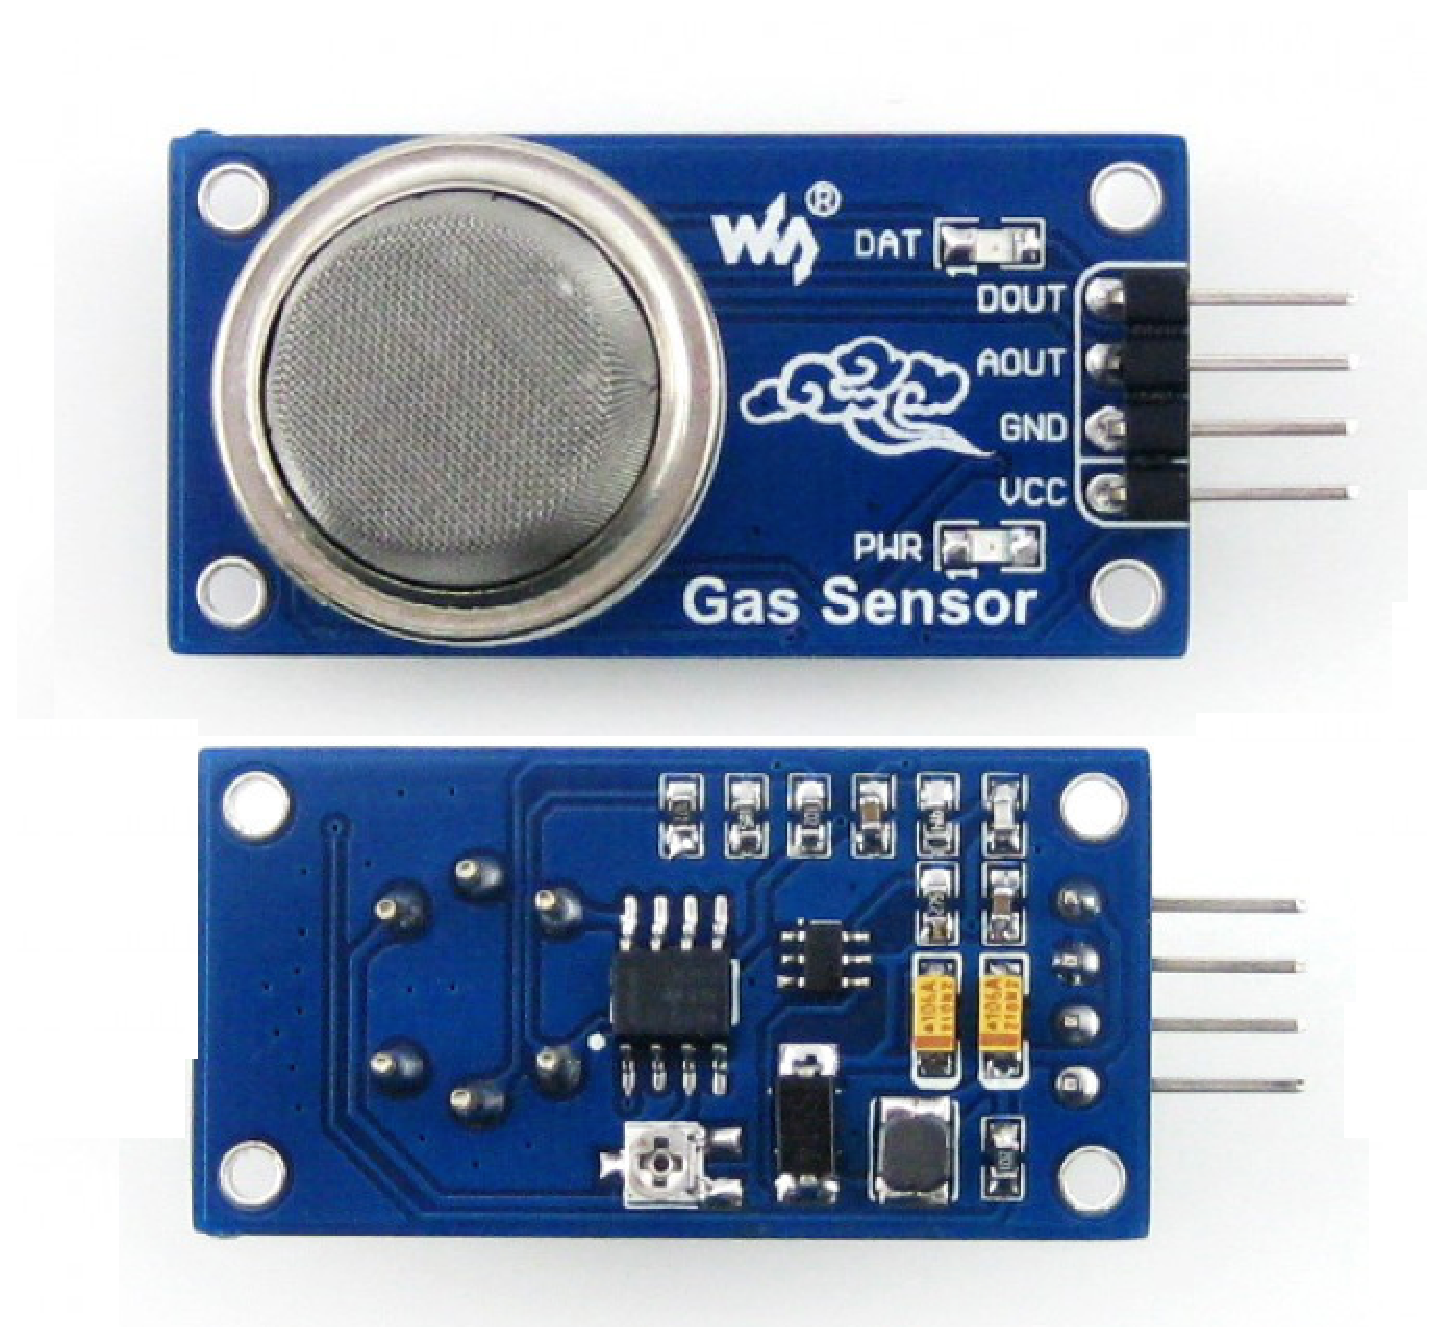
\includegraphics[width=0.7\linewidth]{Figures/Sensors&Rasp/mq-2}
	\caption[gas]{Gas sensor}
	\label{fig:mq2}

\end{figure}

Il sensore di gas (figura~\ref{fig:mq2}) è dotato di un sensore MQ-2 in grado di rilevare la presenza dei seguenti gas:  LPG, propano, idrogeno. Possiede inoltre due led: uno sempre acceso per segnalare la giusta alimentazione del sensore e l'altro per segnalare la presenza di gas (acceso quando vi è gas). Infine, sotto, vi è un trimmer utile alla regolazione della sensibilità del sensore. Vi sono quattro Pin per interfacciarsi.
Le sue caratteristiche tecniche sono: 

\begin{itemize}
	\item Vcc: 2,5$\sim$5V
	\item Output: HIGH o LOW (boolean sensor: 0-1)
\end{itemize}

\newpage

\subsection{Hardware Aggiuntivo}

Abbiamo cercato di realizzare il progetto provando a semplificare il pi\`u possibile la parte hardware.
In particolare ci siamo impegnati ad acquistare moduli (schede provviste di sensori e le resistenze necessarie al loro funzionamento) provvisti di sensore invece dei singoli sensori.

\begin{figure}
	\centering
	\includegraphics[width=0.7\linewidth]{Figures/Sensors&Rasp/breadboard}
	\caption[breadb]{Breadboard}
	\label{fig:bb}
\end{figure}

Questo ci ha permesso di fare a meno di resistenze, led o quant'altro che rendesse necessario l'uso della breadoard (figura~\ref{fig:bb}).
Strumento in grado di effettuare collegamenti, utilizzato molto spesso per realizzare e testare prototipi di circuiti elettrici.

\begin{figure}
	\centering
	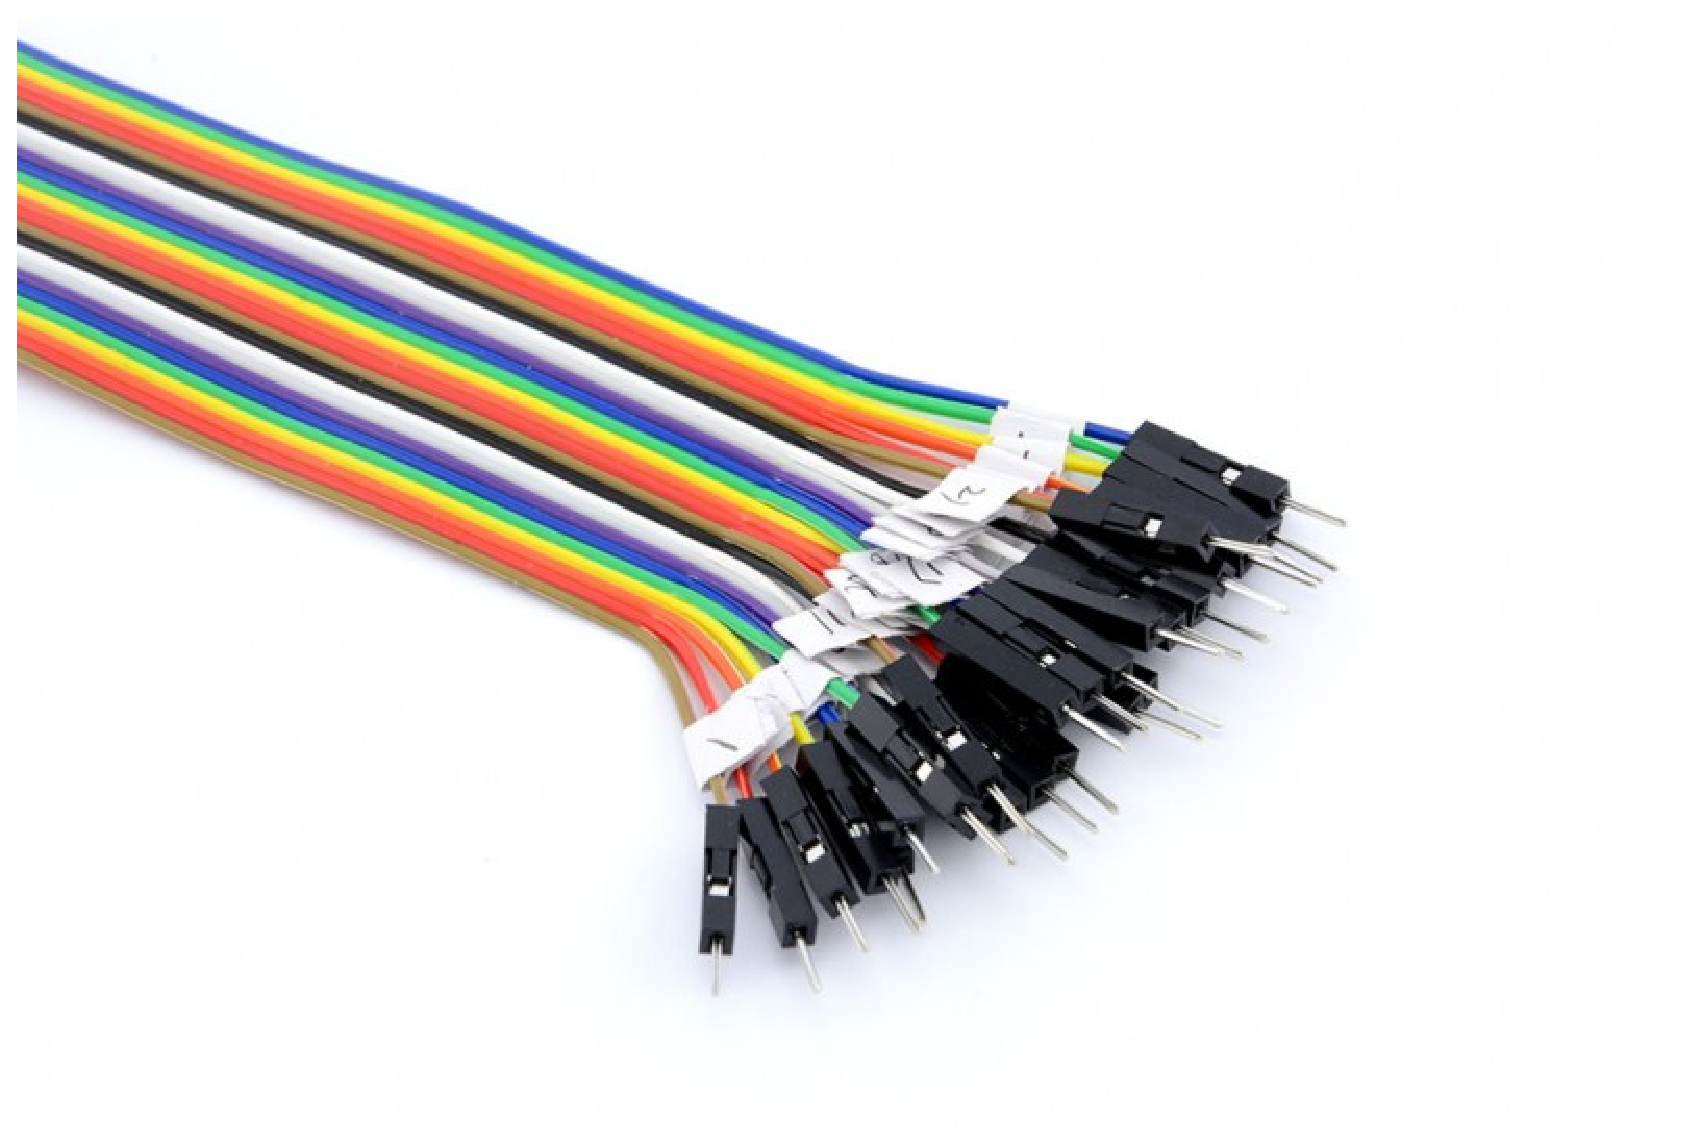
\includegraphics[width=0.7\linewidth]{Figures/Sensors&Rasp/cables}
	\caption[cable]{Cavi di collegamento}
	\label{fig:cables}
\end{figure}

\newpage

Tuttavia \`e stato necessario acquistare un set di cavi di collegamento (esempio in figura~\ref{fig:cables}), cio\`e cavi di metallo rivestiti in plastica, per permettere il collegamento dei vari pin dei sensori alla gpio del Rapberry.

Questi cavi possono essere di tre tipi a seconda delle combinazioni (maschio-maschio, maschio-femmina, femmina-femmina).

Il costo del set di cavi, composto da 50 cavi M-M , M-F, F-F \`e stato di 8€.

\newpage


\section{Analisi dei Requisiti}
\labelsec{ReqAnalysis}
%===========================================================================
\subsection{Casi D'Uso}
\labelssec{UseCases}

\begin{figure}[ht]
\centering
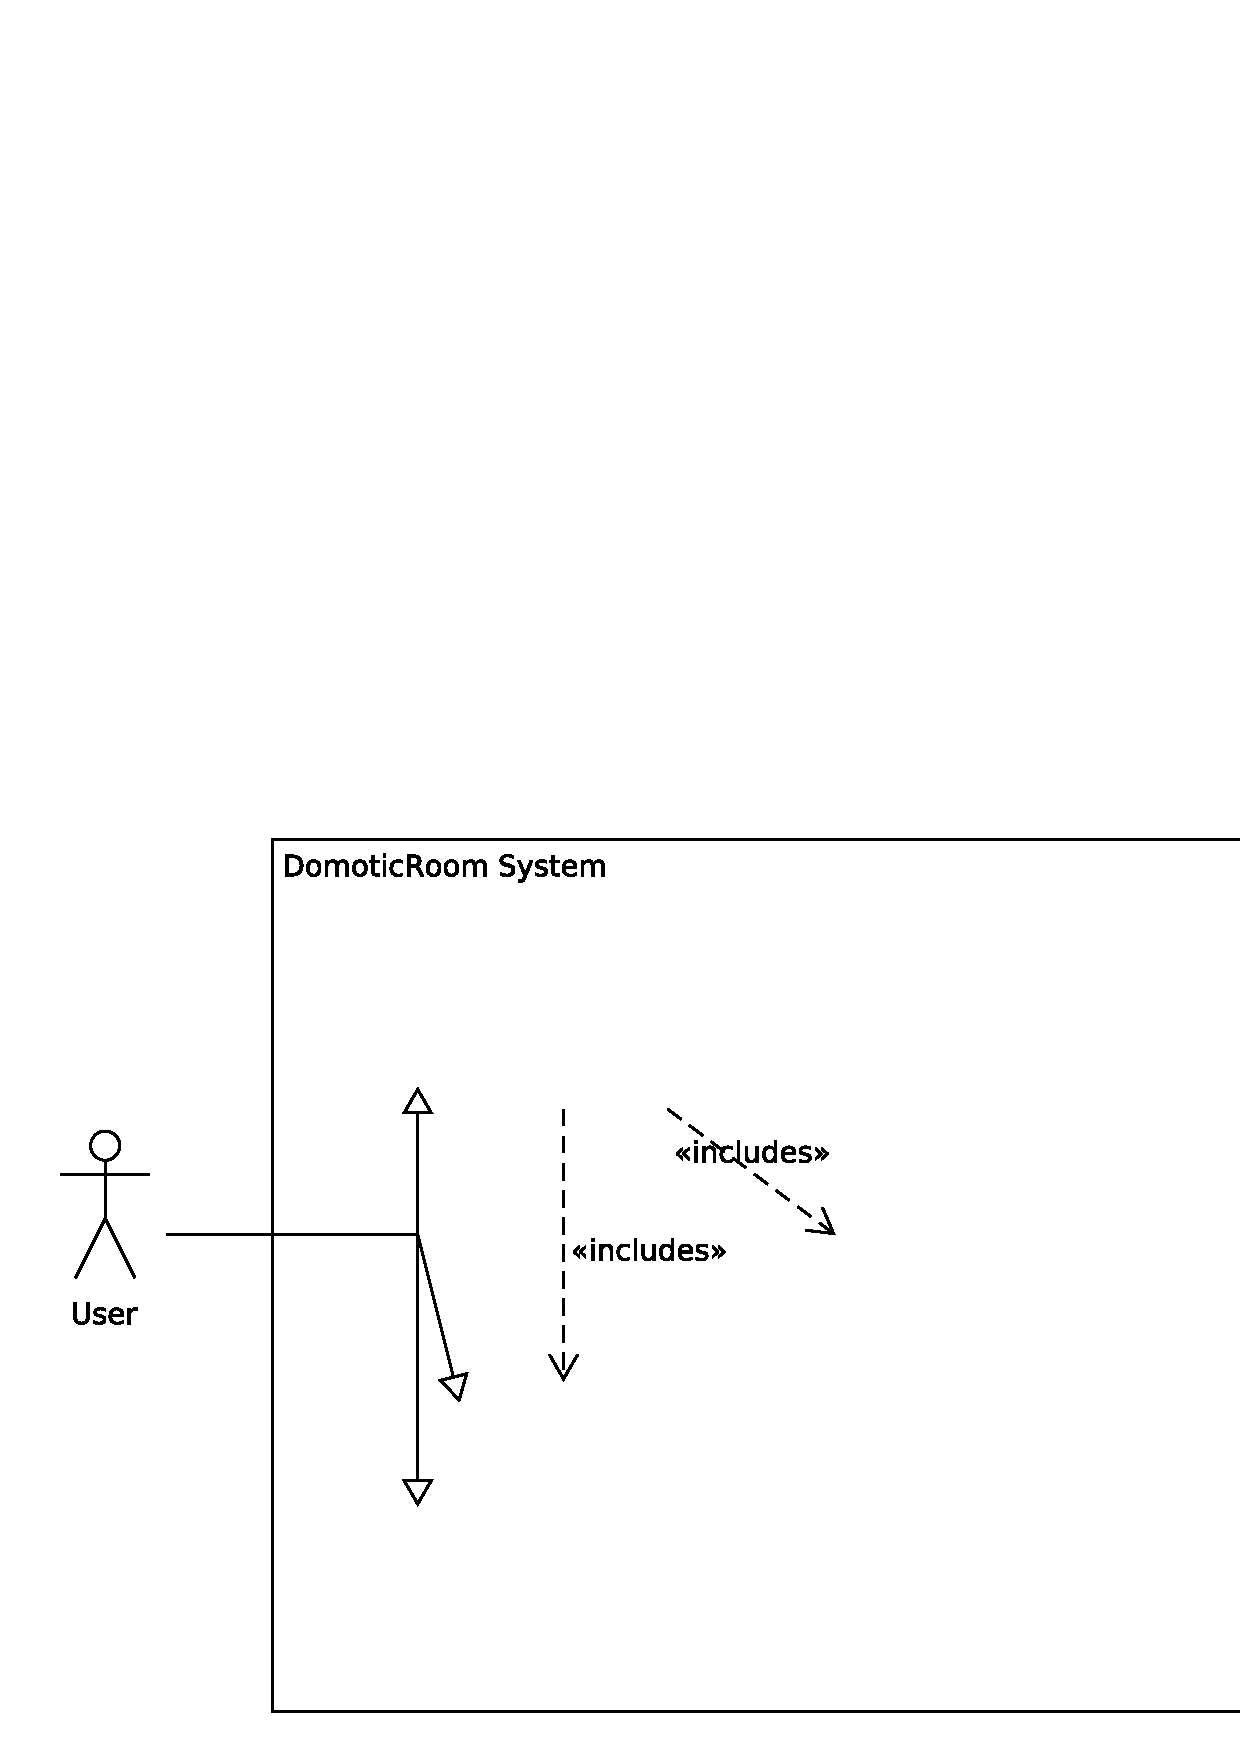
\includegraphics[width=\textwidth]{Figures/UseCases.jpg}
\caption{Casi d'Uso}
\end{figure}

Nell'immagine sopra si possono vedere quali sono le macro operazioni principali effettuate dal sistema e le interazioni con l'esterno. In particolare gli attori che interagiscono con il sistema saranno:

\begin{itemize}
  \item La stanza: con questo attore si intendono i vari parametri che si possono rilevare attraverso i sensori e che quindi saranno di input per il sistema.
  \item Utente: con questo attore rappresenta l'utente che pu\'o interagire con il sistema.
\end{itemize}

Il sistema \'e stato volutamente suddiviso in tre parti distinte con l'idea di seguire un modello MVC dove per\'o la parte di modello non viene aggiornato solamente attraverso l'input inserito dall'utente, ma anche e soprattutto dall'input dei sensori. L'organizzazione hardware ha fortemente influito su questa suddivisione.

\'E inoltre possibile visualizzare le macro operazioni che devono essere effettuate e modellate dal sistema. Si vedano gli scenari di seguito per avere una pi\'u dettagliata visualizzazione dell'interazione tra le varie parti che lo schema sovrastante vuole rappresentare.


\subsection{Scenario}
\labelssec{Scenarios}

In questa sezione verranno illustrati le principali modalit\'a di utilizzo del sistema. Gli scenari elencati di seguito riguardano l'utente e di conseguenza si prevede l'accesso da parte di questo all'interfaccia di input.

Si prevede che il sistema sia opportunamente configurato e settato a livello hardware, senza errori durante la fase di start up.

\subsubsection{Inserimento Range}

\begin{enumerate}
  \item Attraverso un apposito men\'u l'utente \'e in grado di accedere alla funzionalit\'a di settaggio dei range associati ai parametri ambientali.
  \item Il server sa gi\'a i sensori che sono collegati al raspberry appena questi inviano qualche dato e quindi l'utente \'e in grado di visualizzare i controlli relativi ad ogni tipologia di sensore attualmente connesso. Conseguentemente l'utente \'e in grado di modificare tali intervalli.
  \item Al termine della modifica degli intervalli l'utente dovr\'a confermare le modifiche attraverso un'apposito pulsante.
  \item Il sistema mostra un messaggio di conferma o di errore.
\end{enumerate}

\subsubsection{Visualizzazione Stato Realtime}

\paragraph{} All'accesso del sistema l'utente visualizza lo stato realtime dei valori dei sensori ed eventuali notifiche:
\begin{itemize}
  \item Se i valori vanno oltre gli intervalli correnti.
  \item Sullo stato dei sensori, se sono attivi al momento oppure no.
\end{itemize}

In questa modalit\'a l'utente non pu\'o effettuare alcuna operazione.

\subsubsection{Visualizzazione Dati}

\paragraph{} Attraverso un apposito men\'u l'utente \'e in grado di accedere alla visualizzazione dei dati storici dei vari sensori.

\subsection{Modello del Dominio}

In questa sezione vogliamo cercare di modellare le entit\'a inserite all'interno dei requisiti senza fare riferimento alla parte tecnologica e alla parte hardware. In questo modo siamo in grado di decidere noi le interfaccie con cui vogliamo lavorare e costruire la parte software aumentando il disaccoppiamento con la parte fisica e quindi aumentando anche la possibilit\'a di utilizzare volendo lo stesso software su diverse configurazioni. In questo progetto ad ogni modo si utilizzer\'a solamente la configurazione che trovate descritta in questo report.

\paragraph{Suddivisione del Sistema:} visto che \'e emerso gi\'a dai casi d'uso la separazione del sistema in varie parti, ci \'e sembrato giusto iniziare a modellare dividendolo fin da subito in modo da:
\begin{itemize}
  \item semplificare il processo
  \item suddividere il lavoro di implementazione successivamente tra i membri del gruppo.
\end{itemize}

In particolare le parti individuate sono tre:

\begin{itemize}
  \item Sistema Embedded: che nel nostro caso si occuper\'a di catturare, convertire e inviare i dati alle altre parti
  \item Server: Sar\'a la parte che riceve i dati e si occupa di effettuare le varie elaborazioni come ad esempio, il salvataggio dei dati, il calcolo delle statistiche e il controllo dei range. Infine questa parte dovr\'a rendere disponibili i risultati alla parte successiva.
  \item Web site: parte che, prende i risultati dalle parti precedenti e li mostra all'utente rispettando i casi d'uso predecenti.
\end{itemize}

Chiaramente in questa fase tutto viene semplificato e ridotto a poche entit\'a. Questo per\'o non significa che, ogni entit\'a presente negli schemi sottostanti, non si riveli essere poi a sua volta un sottosistema pi\'u complesso.

Lo scopo di questa fase \'e appunto quella ri riflettere, in un primo modello, i requisiti. Poi da questo modello iniziare a sviluppare il progetto cercando di mantenere coerenza nelle interfaccie principali che indicano le interazioni pi\'u importanti.

\subsubsection{Sistema Embedded}

\paragraph{}Per quanto riguarda il sistema embedded \'e necessario prima effettuare delle indagini su come interagire e comunicare con i sensori in modo da modellare adeguatamente il tutto e quindi assicurarsi che in seguito sar\'a semplice riuscire a integrare il tutto con la tecnologia che avremo intenzione di utilizzare. Quindi questa \'e una piccola eccezione che \'e necessario fare a questo livello, anche se in particolare si fa riferimento a un paradigma pi\'u che ad una tecnologia specifica.

\textbf{Il modello di interrogazione dei sensori \'e a polling} di consequenza il nostro modello dovr\'a riflettere questa modalit\'a di interazione. Sfortunatamente questo implica che a livello di modello gi\'a \textbf{un'entit\'a attiva} che si occupa di reperire i valori visto, che in una modalit\'a a polling devo esplicitamente chiedere ai sensori i valori.

\paragraph{Struttura}

\begin{figure}[H]
\centering
\includegraphics[width=\textwidth]{Figures/DomainModel/EmbeddedSystem/Structure.jpg}
\caption{Sistema Embedded, Struttura}
\end{figure}

Dalla struttura si possono subito individuare le entit\'a principali che sono presenti nei requisiti, in particolare la presenza di una specifica gerarchia per i sensori che condividono la stessa interfaccia che consente agilmente di ottenere il valore corrente del sensore. Sono stati inseriti solamente i sensori citati nei requisiti, ma si pu\'o facilmente intuire come qualsiasi tipo di sensore sia facilmente modellabile secondo questa struttura.

Si noti inoltre come viene anche inserita l'entit\'a IConvertor che si occoper\'a di convertire il valore di uno specifico sensore in un'unit\'a pi\'u consona per la sua gestione. Chiaramente questo viene affrontato fin da questo livello perch\'e si immagina l'operazione di conversione come un'operazione quasi istantanea e necessaria.

Infine sono presenti le entit\'a che si occupano, attivamente, di interrogare i sensori ogni intervallo di tempo predefinito e quindi inviarli altrove, In questo caso \'e stato tutto ridotto ad un singolo endpoint, anche se poi possono essere facilmente pi\'u di uno. Come si pu\'o visionare nel commento, l'invio dei dati avviene con una metodologia di tipo \textit{fire and forget}, quindi non avvengono reinvii dei dati e vengono ignorati eventuali errori. Chiaramente tutto questo \'e dovuto all'idea che i cicli di invio siano abbastanza brevi da potersi permettere eventuali perdite.

\paragraph{Interazione}

\begin{figure}[H]
\centering
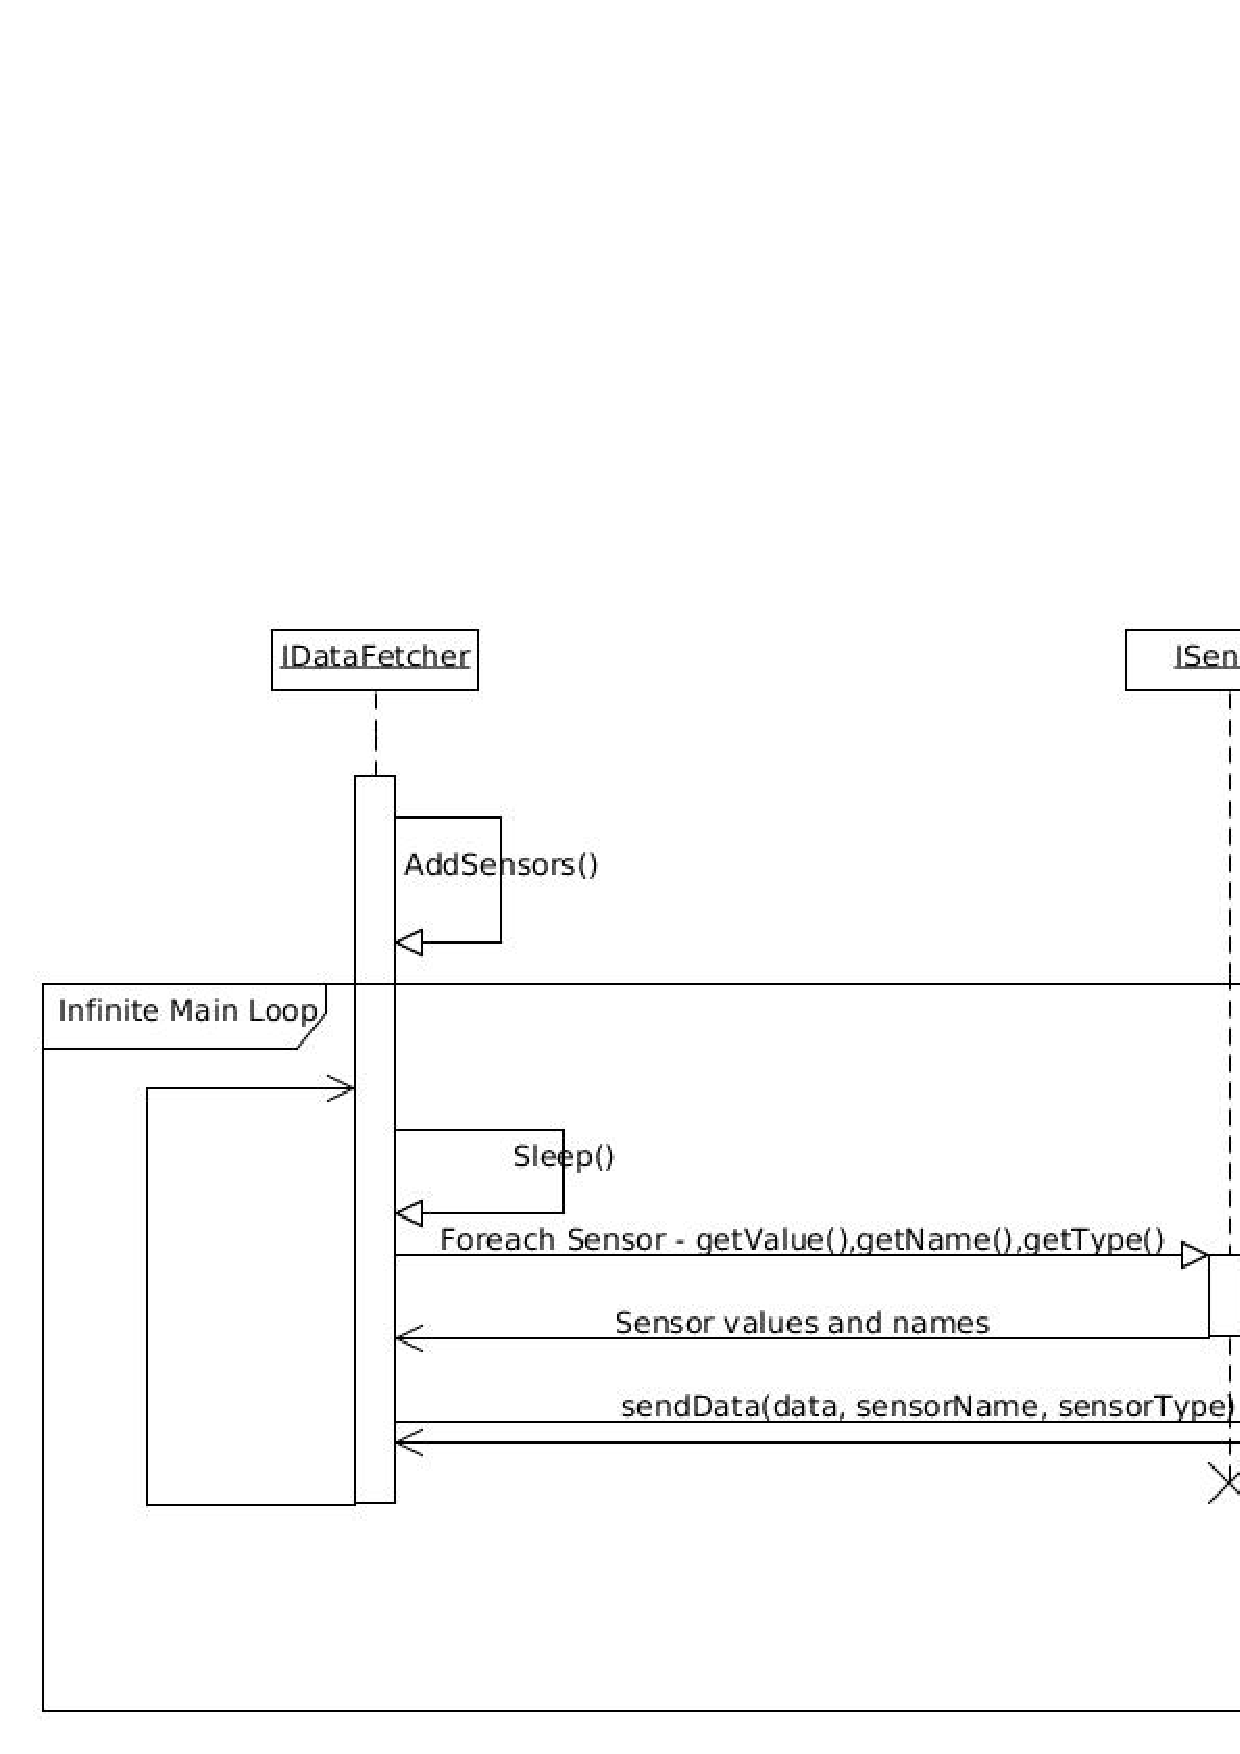
\includegraphics[width=\textwidth]{Figures/DomainModel/EmbeddedSystem/Interaction.jpg}
\caption{Sistema Embedded, Interazione}
\end{figure}

Prima di iniziare si vuole evidenziare come viene riportato solamente un diagramma di interazione perch\'e \'e presente solamente un'entit\'a attiva, ma nel futuro potrebbero esserci pi\'u task e quindi saranno necessari pi\'u diagrammi dell'interazione.

Nello schema di interazione vengono evidenziate le varie fasi del Sistema, in particolare la fase iniziale di setup dove, conoscendo quali sensori sono presenti, questi vengono aggiunti nella memoria dell'entit\'a principale in modo che poi in seguito siano facilmente interrogabili.

Terminata la fase di \textit{Init} inizia il loop infinito che appunto aspetta inizialmente un piccolo lasso di tempo e poi va a interrodage iterativamente tutti i sensori che sono stati aggiunti precedentemente, raccoglie i dati e interroga asincronamente l'entit\'a di invio, per poi ricominciare il ciclo stesso.

\paragraph{Comportamento}

\begin{figure}[H]
\centering
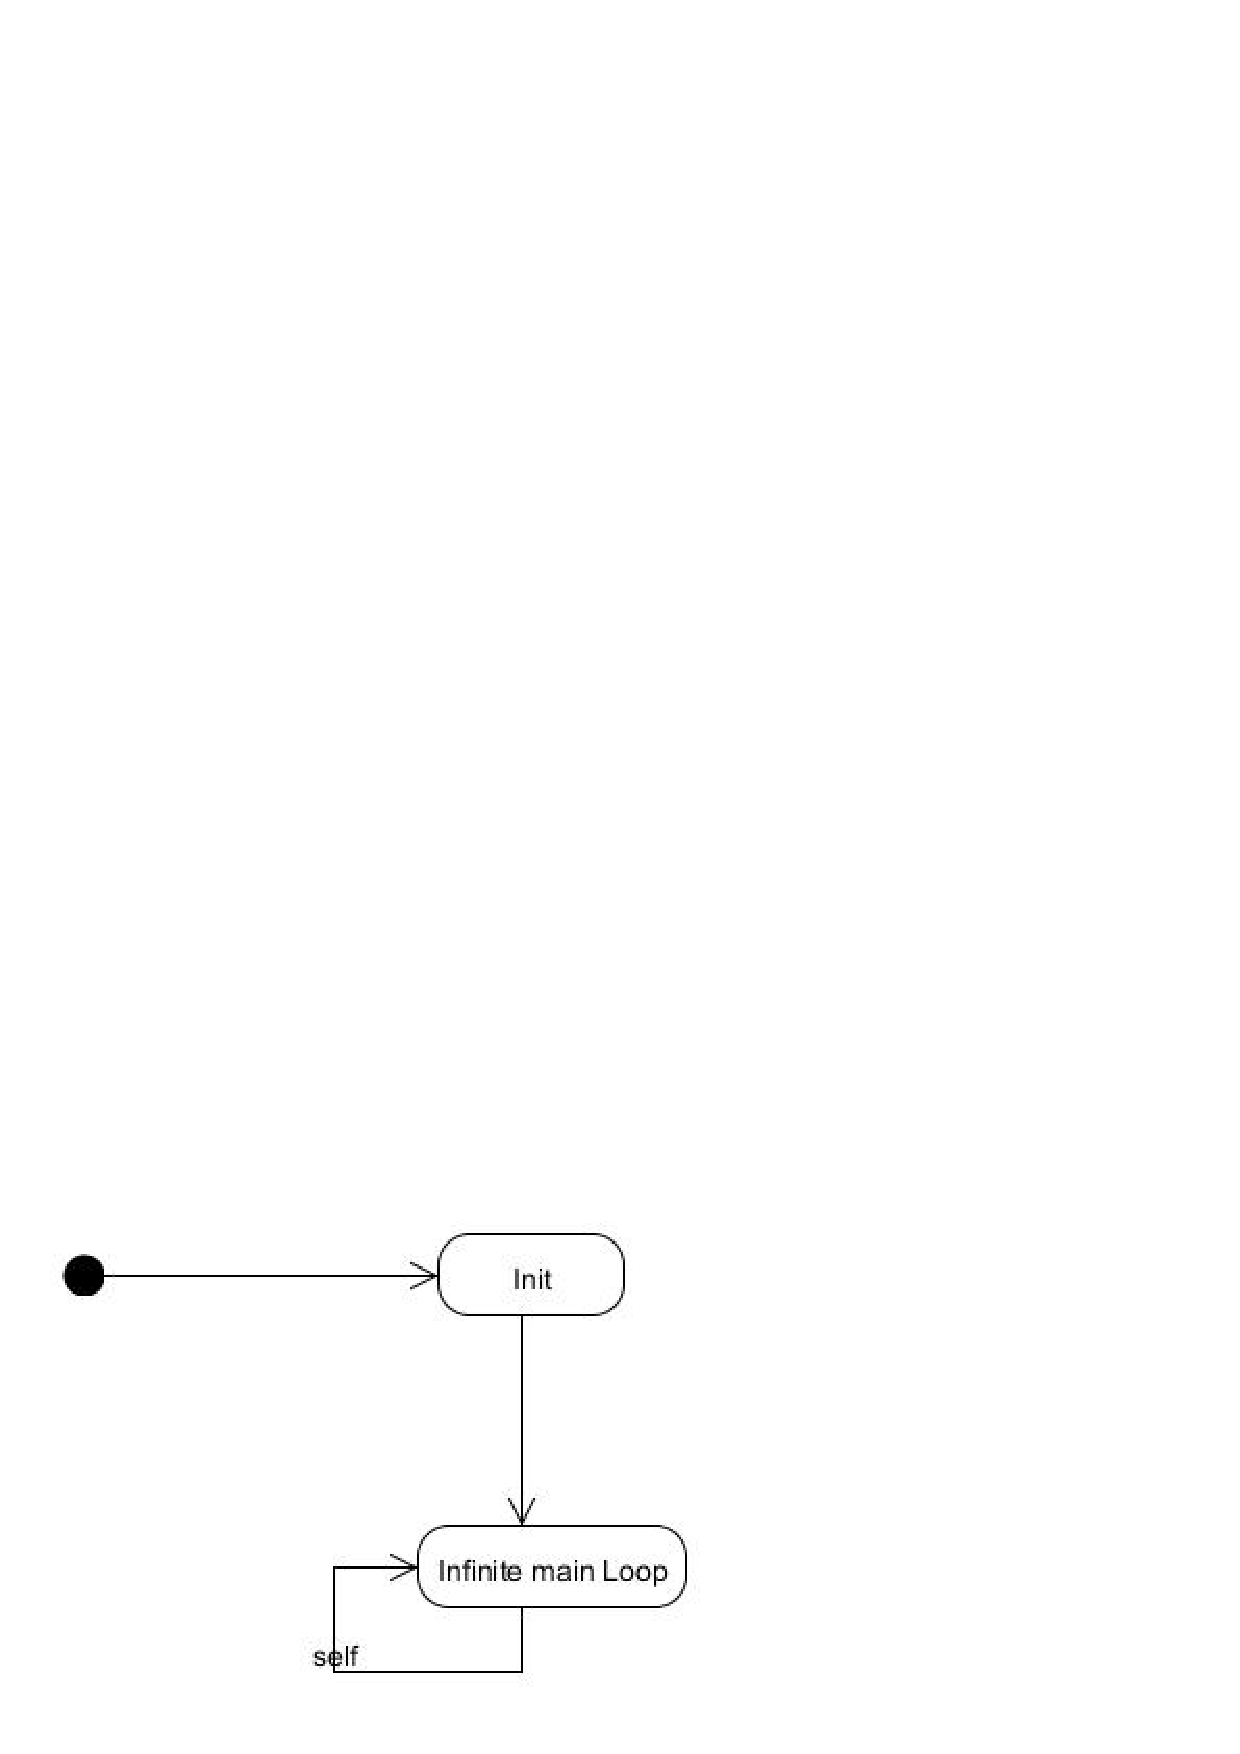
\includegraphics[scale=0.5]{Figures/DomainModel/EmbeddedSystem/Behaviour.jpg}
\caption{Sistema Embedded, Comportamento}
\end{figure}


Nel diagramma del comportamento semplicemente viene riportato quanto \'e stato precedentemente discusso semplicemente attraverso una state machine.

\subsubsection{Server}

\paragraph{}La parte server \'e quella pi\'u importante di tutto il sistema in quanto \'e quella che concentra tutta la logica applicativa del sistema stesso.

\begin{figure}[pH]
\centering
\includegraphics[width=\textwidth,height=\textheight,keepaspectratio]{Figures/DomainModel/Server/Structure.jpg}
\caption{Server, Struttura}
\end{figure}

\afterpage{\clearpage}

\newpage

\paragraph{Struttura}

Le entit\'a principali di questo schema sono:
\begin{itemize}
  \item IPersistentStore, che si occuper\'a di salvare opportunamente i dati provenienti dai sensori e dall'utente
  \item IDataReceiver, che sar\'a sempre in ascolto di ogni messaggio proveniente dal sistema embedded e quindi notificher\'a opportunamente il sistema ad ogni nuovo arrivo
  \item IPresentator che si occuper\'a di ottenere i dati necessari per le viste da mostrare all'utente quanto una nuova richiesta viene inoltrata.
\end{itemize}

Chiaramente ogniuna di queste entit\'a \'e in parte citata nei casi d'uso.

Si veda i diagrammi dell'interazione per i dettagli di come avviene la comunicazione di tutte queste entit\'a al fronte di garantire il funzionamento e il soddisfacimento dei requisiti.

\paragraph{Interazione}

\begin{figure}[H]
\centering
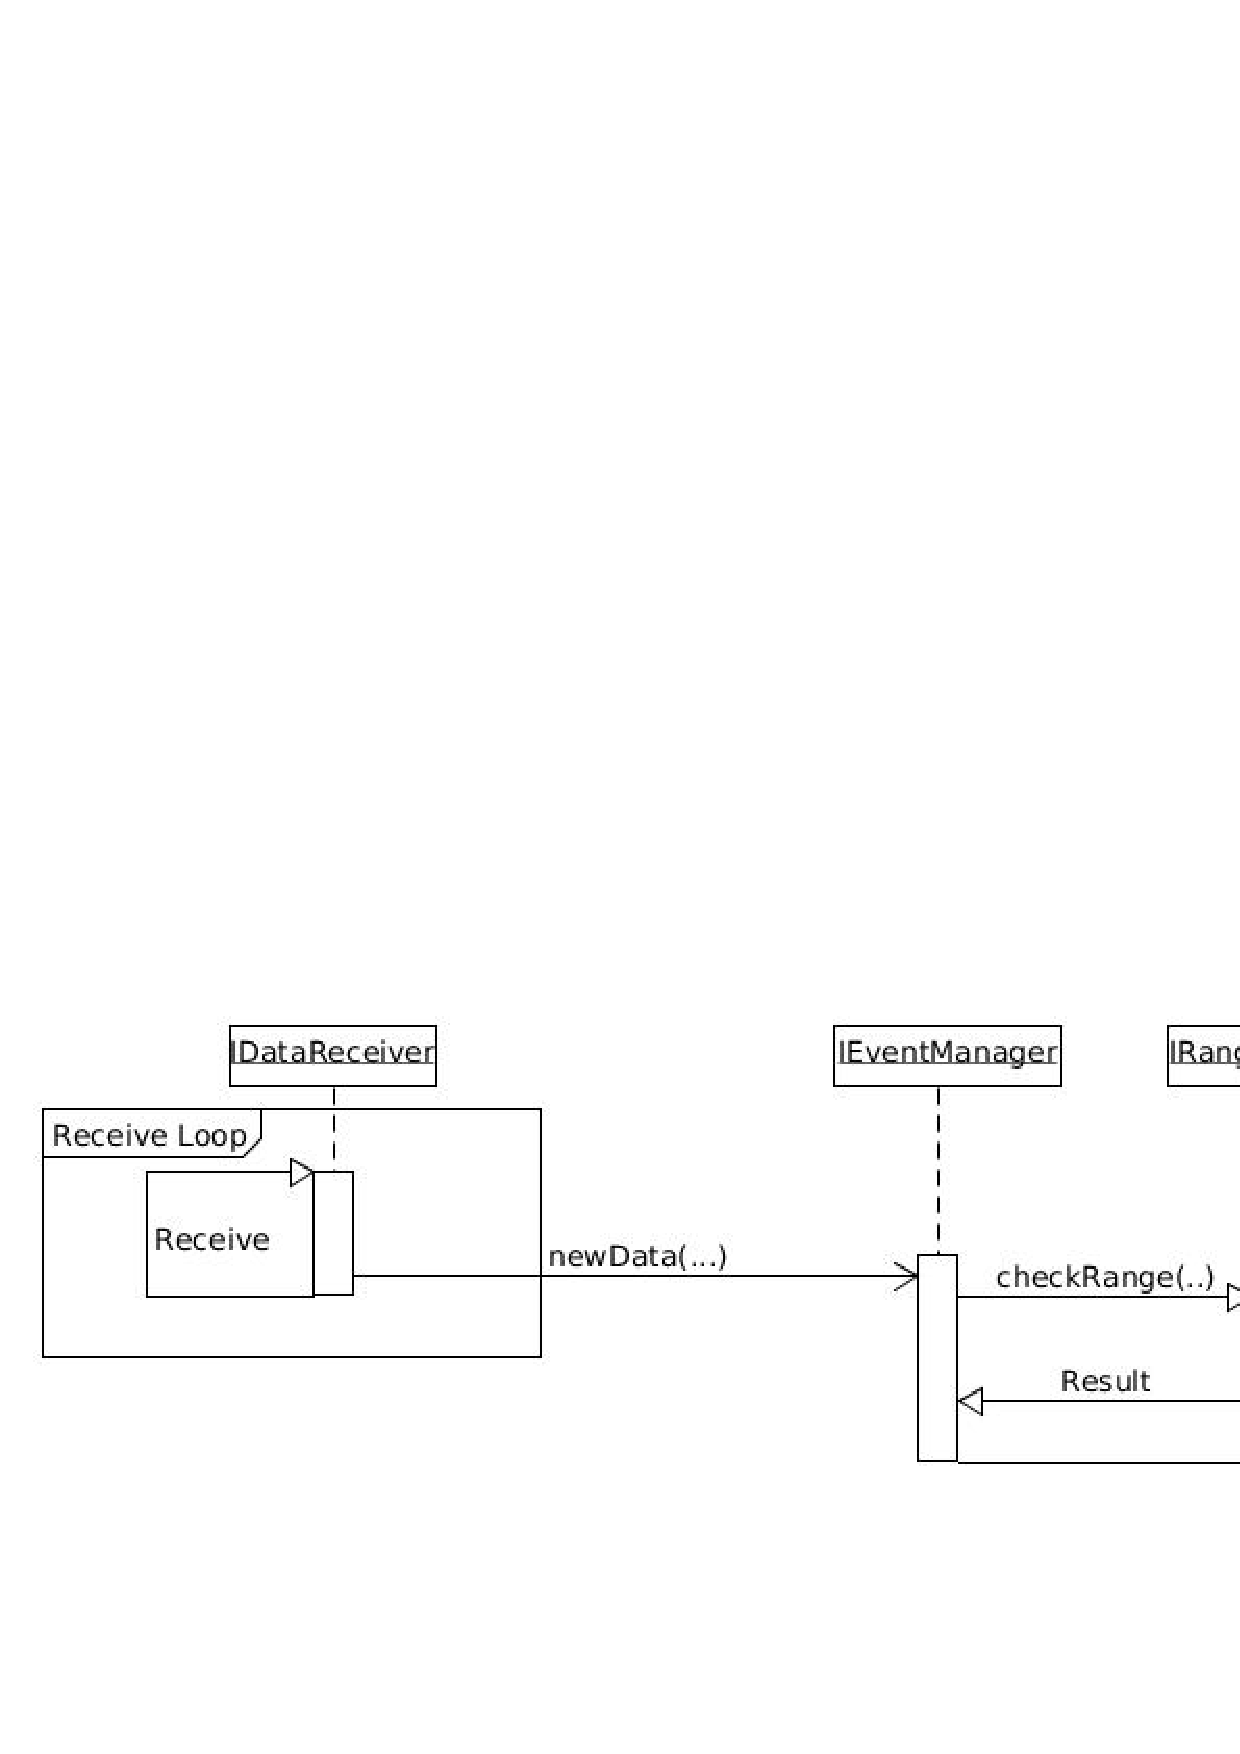
\includegraphics[width=\textwidth]{Figures/DomainModel/Server/NewDataInteraction.jpg}
\caption{Server, Comportamento, Dati dai Sensori}
\end{figure}

Abbiamo deciso di omettere la parte di inizializzazione del sistema in questa fase anche perch\'e sar\'a meglio defita nell'analisi del problema dovendo aggiungere entit\'a che non sono direttamente correlate con i requisiti principali ma con requisiti non funzionali.

Nello schema sovrastante si pu\'o osservare l'interazione nel caso i sensori emettano un nuovo valore. Si vuole porre particolare enfasi su come l'entit\'a che riceve i dati rimane sempre in ascolto di nuovi arrivi delegando, tramite una chiamata asincrona alle altre entit\'a il compito di salvare i dati appena arrivati.

\noindent\rule[0.5ex]{\linewidth}{1pt}

\begin{figure}[H]
\centering
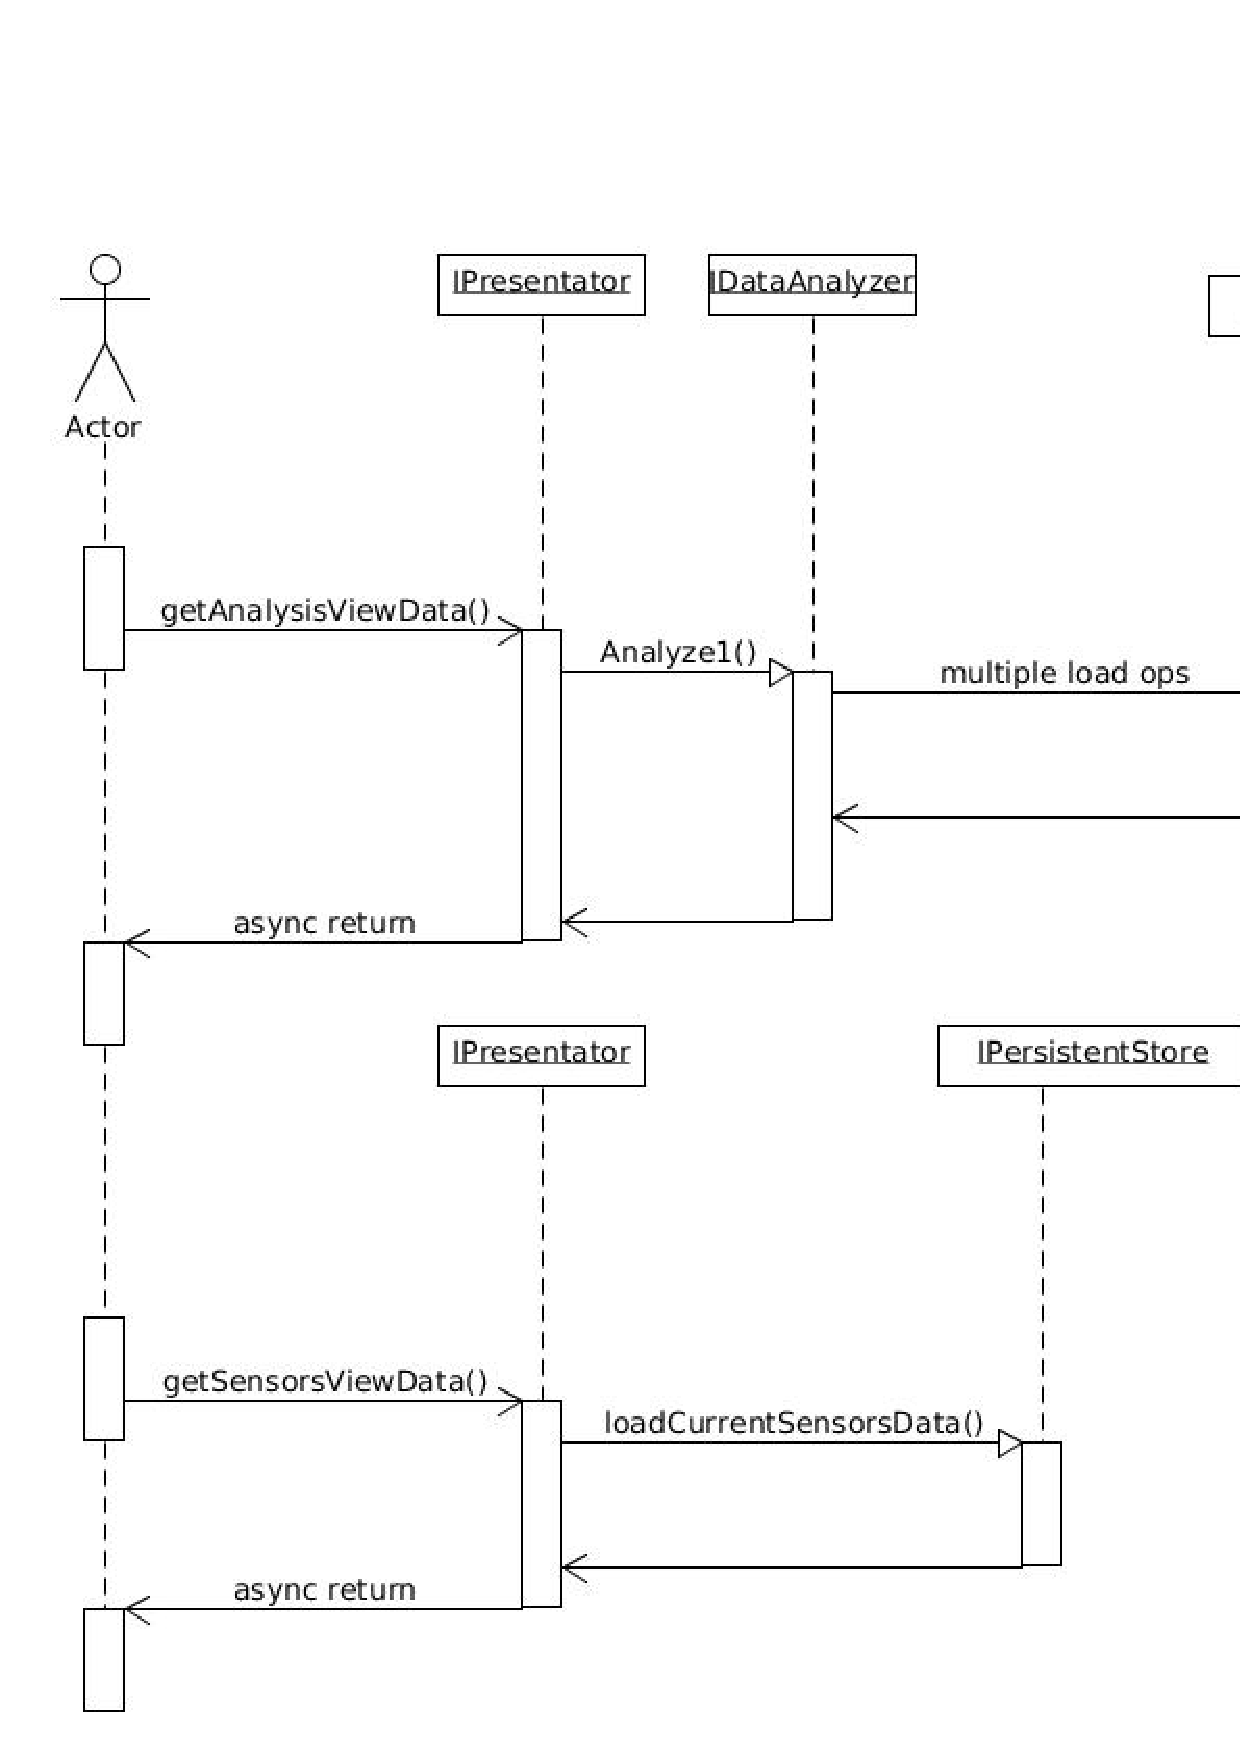
\includegraphics[width=\textwidth]{Figures/DomainModel/Server/GetOperationInteraction.jpg}
\caption{Server, Comportamento, Richiesta Visualizzazione Dati}
\end{figure}

In quest'altro schema dell'interazione si pu\'o osservare che entit\'a vengono conivolte a fronte di una chiamata di visualizzazione dati da parte dell'utente. Anche in questo caso la chiamata iniziale \'e stata effettuata in maniera asincrona in modo da lasciare libero il sistema di rispondere ad eventuali altre richieste e gestirle concorrentemente.

\noindent\rule[0.5ex]{\linewidth}{1pt}

\begin{figure}[H]
\centering
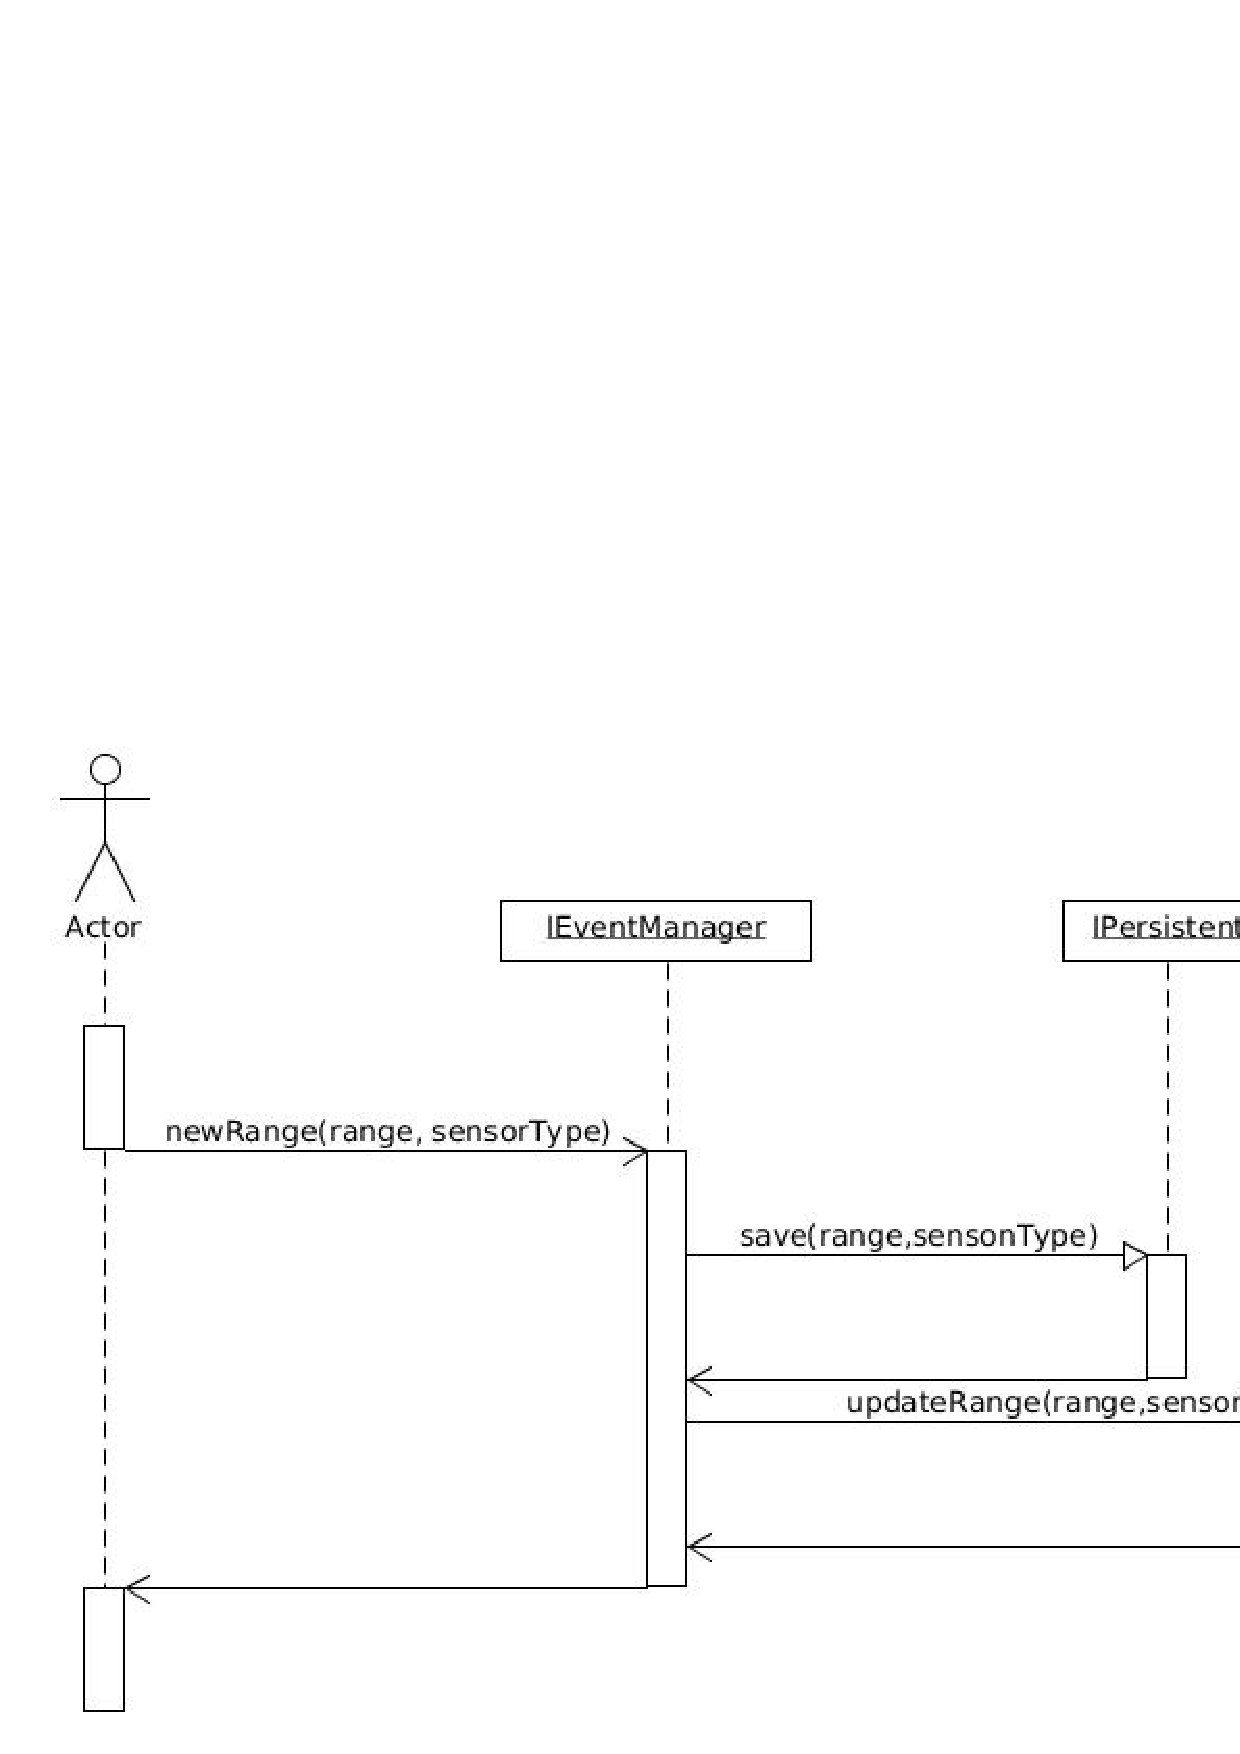
\includegraphics[width=\textwidth]{Figures/DomainModel/Server/NewRangeInteraction.jpg}
\caption{Server, Comportamento, Nuovo Range}
\end{figure}

In questo caso invece viene illustata l'interazione per quanto riguarda la richiesta da parte dell'utente dell'inserimento di un nuovo range. Si vede come la chiamata questa volta arriva all'entit\'a che gestisce gli eventi essendo questo effettivamente un caso incui avviene un cambiamento nei dati e quindi tutto va gestito appropriatamente per evitare i conflitti.

\paragraph{Comportamento}

\subsubsection{Web Site}

\paragraph{}Dopo un'attenta analisi abbiamo ritenuto superflua la necessit\'a di modellare e analizzare la parte di visualizzazione in quanto non \'e effettivamente presente nessuna business logic ma solamente la parte che effettua le richieste di dati alle parti precedenti e visualizza tutto su schermo.

La documentazione relativa a questa parte si limiter\'a solamente a come utilizzare poi il software attraverso l'interfaccia.

Possiamo per\'o pensare di definire i link a cui l'interfaccia dovr\'a rispondere appropriatamente attraverso una pagina web. Questo ci consente di impostare comunque dei test che esulano dal contenuto della pagina, ma ci garantiscono che questa sia effettivamente online in maniera automatica.

gli URL scelti sono:
\begin{itemize}
  \item \textit{http://...../DomoticRoom/Status}
  \item \textit{http://...../DomoticRoom/NewRange}
  \item \textit{http://...../DomoticRoom/Analysis}
\end{itemize}

\subsection{Piani di Test}

In questa fase saranno presenti i piani di test che vengono costruiti sulla base dei modelli precedenti, ancora privi di implementazione. Ci\'o \'e possibile perch\'e a questo punto abbiamo gi\'a individuato le interfaccie delle entiti\'a principali e le loro operazioni pubbliche.

Chiaramente a questo punto la maggior parte dei test non possono funzionare perch\'e manca l'implementazione. Anche in questa fase si divide il tutto sulle 3 parti precedenti.

\subsubsection{Sistema Embedded}
\subsubsection{Server}
\subsubsection{Web Site}


\section{Analisi del Problema}
\labelsec{ProblemAnalysis}
%===========================================================================

\paragraph{Assunzioni}
Prima di iniziare l'analisi del problema abbiamo ritenuto neccessario effettuare delle assuzioni riguardanti al paradigma che ci consentirebbe di effettuare un prodotto di qualit\'a migliore e con meno sforzi.

Il paradigma di programmazione di riferimento \'e il \textit{reactive programming} perch\'e la concezione di flusso di dati \'e proprio quello che ci interessa modellare in quanto anche nel nostro sistema sar\'a presente un flusso di dati dal client al server. Per la comunicazione attraverso la rete questo ci consente di sfruttare chiamate asincrore aumentando il disaccoppiamento tra client e server.

Per questo abbiamo deciso di utilizzare per i dati un database NoSQL per via dell'estremo dinamismo, in quanto ci consente di aggiungere dei campi anche in seguito e miglioramento di performance nell'accesso a dati che normalmente richiederebbero dei join.

Per ulteriori informazioni pi\'u dettagliate sul paradigma si rimanda ad un'altra sede. 

\subsection{Architettura Logica}

Per la costruzione dell'architettura logica ci si baser\'a ovviamente sulla precedente analisi dei requisiti in modo da mantenere il contatto con questi e non rischiare di uscire fuori specifica. Anche in questo caso si andr\'a separare l'analisi in due parti:

\begin{itemize}
\item Embedded System
\item Server e Website
\end{itemize}

La parte del website \'e stata incorpata direttamente nella parte server proprio per la sua assenza di business logic.

\paragraph{Modellazione Reactive}

Prima di iniziare a costruire la modellazione sulla base del paradigma appena citato \'e necessario capire come fare a modellare lo stream stesso all'interno della nostra architettura logica, conseguentemente si \'e deciso di utilizzare i \textit{marable diagrams}. Questi sono una rappresentazione di come il flusso di dati nel tempo avviene e quali tipologie di trasformazioni consentono di effettuare.

Con questi schemi ci viene concesso ancora una volta di concentrarci prima sul ''cosa'' e non sul ''come'' che invece viene delegata alla parte progettuale, dove si cercher\'a effettivamnete di implementare il risultato finale dell'analisi


\subsection{Gap di Astrazione}

In questa sezione aggiungeremo tutti i tipi di astrazioni che sono richieste per affrontare il progetto e che non sono direttamente fruibili attraverso la tecnologia di riferimento.

\begin{enumerate}
  \item Web Server: Vista la necessit\'a di comunicare attraverso la rete \'e necessario che si utilizzi un paradigma a message-passing o attraverso chiamate asincrone, soprattutto per la comunicazione che avviene tra il raspberry e il server.
  \item Continuous Integration, Testing and collaborative source control: Lavorando in gruppo sullo stesso repository \'e necessario impostare il lavoro affinch\'e sia possibile effettuare le modifiche in maniera indipendente gli uni dagli altri e allo stesso modo sia possibile controllare automaticamente che i test predisposti e le modifiche effettuate siano coerenti con le specifiche e che il building del progetto sia in ogni caso garantito.
  \item{Paradigmi Eterogenei}: si \'e deciso di utilizzare dei paradigmi diversi dal OOP classico e questo pu\'o portare a problematiche di utilizzo, per via dell'inesperienza e comunque non vengono fornite direttamente dal linguaggio e quindi vanno trovate soluzioni al problema.
\end{enumerate}

\subsection{Analisi dei Rischi}

In questa sezione vanno elencati invece i rischi che si possono intraprendere in un progetto di questo tipo e quindi formalizzarli fin da subito, prima di eseguire l'effettiva realizzazione dello stesso in modo da poterli affontare e discutere preventivamente per essere pronti se questi si verificano.

\begin{itemize}
  \item Aumento dei Costi: \'e necessario porre particolare attenzione alla struttura hardware del sistema e di come i singoli componenti vanno ad interconnettersi assieme per evitare che si debbano affrontare dei costi aggiuntivi, una volta che il progetto \'e gi\'a avviato, causati da una qualche mancanza o per via di un'estensione del progetto in corso d'opera.
  \item Quantitativo della memoria: l'adozione di un database NoSQL porta con se un certo livello di ridondanza e quindi questo pu\'o portare ad un aumento di utilizzo della memoria e di spazio. Il tutto va valutato accuratamente durante il progetto, magari attraverso una serie di prove in base a come \'e stutturato il dato inizialmente. Se il rischio quindi \'e reale e quanto \'e critico.
  \item Integrazione tra le tecnologie: un possibile rischio riguarda la difficolt\'a nell'integrare tutte le tecnologie che devono essere sfruttate nel progetto per riuscire a colmare l'abstraction gap e quindi riuscire a completare il progetto attraverso l'analisi appena completata.
\end{itemize}


\section{Work Plan}
\labelsec{WorkPlan}
%===========================================================================



\section{Project}
\labelsec{Project}
%===========================================================================
\subsection{Database}
Per la gestione del database si \'e scelto di utilizzare un database NoSql, nell'accezione MongoDB\cite{MongoDB}. In questa sede non si discuteranno i vantaggi, gli svantaggi o le particolarit\'a di questa tecnologia in quanto \'e stato fatto gi\'a ampiamente durante il corso. Di seguito si riportano gli schemi dei documenti che sono stati salvati, le collezioni e il significato di alcuni dei valori inseriti.

\begin{center}
\textbf{Collection Ranges}
\end{center}

In questa collezione di documenti vengono raggruppati tutti i documenti relativi ai ranges che sono da controllare. In particolare sono stati individuati due tipologie di range in base alla tipologia di sensori.

\begin{itemize}
  \item Si/No: Per quella tipologia di sensori che non forniscono effettivamente dei valori ma che notificano solamente la presenza o l'assenza di un particolare elemento come il GAS o il movimento.
  \item  Valore: validi quando un sensore effettivamente serve una misurazione di una grandezza, come ad esempio la temperatura. In questo caso \'e utile sapere se questa grandezza rimane all'interno di determinati range.
\end{itemize}
 
\begin{figure}[ht]
\centering
\includegraphics[width=\textwidth,natwidth=610,natheight=642]{Figures/DataStructures/RangesBoolean.png}
\caption{Documento dei Ranges Booleani}
\end{figure}


\begin{figure}[ht]
\centering
\includegraphics[width=\textwidth,natwidth=610,natheight=642]{Figures/DataStructures/RangesValues.png}
\caption{Documento dei Ranges di Valori}
\end{figure}

Si vuole far notare come sia comunque sempre presente un attributo di tipo data in modo da poter filtrare i range in base al tempo di inserimento e la presenza di un valore numerico che in questo caso rappresenta il tipo di range.

Per indicare il tipo di range si riporta il listato scala che indica tale tipologia.

\begin{figure}[ht]
\centering
\includegraphics[scale=0.5,natwidth=610,natheight=642]{Figures/DataStructures/Ranges.png}
\caption{Valore numerico dei Ranges}
\end{figure}

\begin{center}
  \textbf{Collertion Sensors}
\end{center}

Per quanto riguarda la collezione dei sensori si utilizza un'apposita collection. Questa non sar\'a modificata spesso, e serve principalmente per eventuali evoluzioni del progetto, in modo che sia gi\'a presente. Anch'essi sono dotati di di tipo come i range e, per questa implementazione, i tipi coincidono. A livello di progetto per\'o si \'e deciso di mantenerli separati nel caso in un futuro questi divergano. Inseriamo di seguito un'immagine che rappresenta come \'e strutturato un documento di un sensore.

\begin{figure}[ht]
\centering
\includegraphics[scale=0.5,natwidth=610,natheight=642]{Figures/DataStructures/Sensors.png}
\caption{Rappresentazione a DB dei Sensori}
\end{figure}

\begin{center}
\textbf{Collection Data}
\end{center}

Per quanto riguarda la rappresentazione dei dati raccolti, anche in questo caso sono presenti 2 tipologie di dati:
\begin{itemize}
\item Dati Corretti: cio\'e quella tipologia di dati che rientrano all'interno del range prestabilito per la loro tipologia.
\item Dati Incorretti: quelli che invece non rientrano nella tipologia corretta e quindi vanno a violare il range attivo.
\end{itemize}

Come si pu\'o osservare il primo tipo \'e pi\'u semplice e ingloba i precedenti. Di seguito come fatto in precedenza si indica un esempio di struttura di un dato corretto e non corretto.

\begin{figure}[ht]
\centering
\includegraphics[scale=0.5,natwidth=610,natheight=642]{Figures/DataStructures/DataNoViolation.png}
\caption{Dato Corretto salvato in database}
\end{figure}

Come si pu\'o osservare \'e stato comunque inserito un valore per la violazione a \textit{null} in modo da poter distinguere meglio i dati violati da quelli invece corretti.

\begin{figure}[ht]
\centering
\includegraphics[scale=0.5,natwidth=610,natheight=642]{Figures/DataStructures/DataViolation.png}
\caption{Dato Non Corretto salvato in database}
\end{figure}

In questo caso appunto il valore della violazione non e' piu' nullo ma contiene un semplice campo \textit{delta} che indicher\'a la differenza rispetto al range. In particolare questo sar\'a positivo se il valore registrato supera il range attuale, negativo se invece \'e troppo basso o booleano se il tipo di sensoristica e quindi anche di range \'e booleano.

\subsection{Introduzione All'Architettura di Progetto}

Nelle prossime sezioni si vuole inserire le modifiche che sono state fatte alla architettura logica appena introdotta, ma cercando di evitare di ripetere aspetti che non sono effettivamnete cambiati. Di conseguenza si \'e deciso di riportare solamente quegli aspetti che sono stati modificati in base alle scelte tecnologiche effettivamente fatte.\\
In ogni caso si \'e deciso di cercare il pi\'u possibile di sfruttare quanto gi\'a \'e stato concordato dagli analisti cercando di effettuare meno modifiche possibili all'architettura.

\subsection{Struttura}
\subsection{Interazione}

In questa parte si riporta la tecnologia che si \'e utilizzata per effettuare l'interazione che si \'e analizzata e indicata in fase di analisi, lo stream. In particolare si \'e notato che, il framework play\cite{PlayFramework} gi\'a gestisce attraverso delle sue strutture la possibilit\'a di operare attraverso stream di dati. Questa possibilit\'a \'e stata introdotta dal framework per gestire meglio dati parziali o casi che richiederebbero molto tempo, come ad esempio un'upload di file cospiquo. Nonostante tutto per\'o questo rientra nelle nostre necessit\'a e quindi ci avvarremo di questa astrazione per risolvere il nostro problema. Si riporta in bibliografia quindi la documentazione del framework che spiega il funzionamento di \textit{Enumerators,Iteratees e Enumeratees.} \cite{PlayStreaming}

\subsection{Comportamento}


\section{Implementazione}
\labelsec{Implementazione}
%===========================================================================

In questa fase bisognerebbe riportare il codice che implementa le varie parti, per\'o, per non appesantire troppo questa relazione che vuole essere una spiegazione alle scelte progettuali e di anali effettuate, si rimanda al lettore la revisione del codice. Di seguito si inserisce il link al repository contenente tutti i sorgenti del progetto stesso, nonch\'e il sorgente di tale documentazione.

\url{https://github.com/benkio/DomoticRoom}


\section{Testing}
\labelsec{Testing}
%===========================================================================

\subsection{Server}

Per quanto riguarda la parte di testing del server si sono implementati e impostati per lo sviluppo alcuni test unitari dell'applicativo. Il codice si pu\'o visionare all'interno dell'apposita cartella di test.

Particolare attenzione si \'e poi posta per i test di integrazione incui si \'e sviluppato un semplice script in fsharp che consente di simulare l'invio di dati dai valori random, strutturati come indicato nella sezione del progetto, all'endpoint specifico del server che si occupa di ricevere e salvare correttamente i dati. Questo ha consentito di parallelizzare al meglio il lavoro tra i membri del gruppo inquanto \'e possibile testare l'applicativo senza dover ottenere dei dati reali e conseguentemente impostare tutta l'infrastruttura ed inoltre ha impostato uno standard da seguire per l'invio dei dati verso il server che i client devono seguire affinch\'e non si verifichino problemi. Anche questo script e' presente nel repository con le relative dipendenze.


\input{11_Deployment.tex}

\input{12_Maintenance.tex}

%%% \begin{itemize}
%%% \item Titolo di studio:\\ \\
%%% \item Interessi particolari:\\ \\
%%% \item Ha sostenuto fino ad oggi il seguente numero di esami:\\ \\
%%% \item Deve ancora sostenere i seguenti esami del I anno:\\ \\
%%% \item Prevede di svolgere un tirocinio presso:\\ \\
%%% \item Prevede di laurearsi nella sessione:\\ \\
%%% \item Intende proseguire gli studi per conseguire: \\  \\  \\
%%%   	presso la sede universitaria di: \\ \\
%%% \item Intende entrare subito nel mondo del lavoro presso : \\ \\
%%% \end{itemize}

 
\appendix


\bibliographystyle{abbrv}
\bibliography{biblio}

\end{document}
